\chapter{Cálculo de raíces de una función\\ Methods for calculating the roots of a function }


\begin{paracol}{2}
\section{Raíces de una función}
Se entiende por raíces de una función real $f(x):\mathbb{R} \rightarrow \mathbb{R}$. los valores $x=r$ que satisfacen, $f(r)=0$

El cálculo de las raíces de una función, tiene una gran importancia en la ciencia, donde un número significativo de problemas pueden reducirse a obtener la raíz o raíces de una ecuación.

La obtención de la raíz de una ecuación es inmediata en aquellos casos en que se conoce la forma analítica de su función inversa $f^{-1}$, ($f(x)=y\Rightarrow f^{-1}(y)=x$). En este caso, $r=f^{-1}(0)$. Por ejemplo,
\switchcolumn
\section{Roots of a function}
The roots of a real function $f(x):\mathbb{R} \rightarrow \mathbb{R}$ are those values $x = r $ for which $f(r) = 0$

Obtaining the roots of a function is of great interest because many scientific problems could be reduced to the calculus of the root or roots of a function.

Obtaining the root of a function is trivial for those cases in which we know the inverse function $f^{-1}$, ($f(x)=y\Rightarrow f^{-1}(y)=x$). In this case, $r=f^{-1}(0)$. For instance,  
\end{paracol}

\begin{align*}
f(x)&=x^2-4\\
f^{-1}(y)&=\pm\sqrt{y+4}\Rightarrow r=f^{-1}(0)=\pm 2\
\end{align*}

\begin{paracol}{2}
Sin embargo, en muchos casos de interés las funciones no pueden invertirse.  Un ejemplo, extraído de la física es la ecuación de Kepler para el cálculo de las órbitas planetarias,
\switchcolumn
Nevertheless, there are many cases where functions cannot be inverted. An example from physics is Kepler's equation for planetary orbits.  
\end{paracol}
\begin{equation*}
x-a\sin(x)=b
\end{equation*}
\begin{paracol}{2}
Donde $a$ y $b$ son parámetros conocidos y se desea conocer el valor de $x$. La solución de la ecuación de Kepler es equivalente a obtener las raíces de la función $f(x)=x-a\sin(x)-b$. (La figura \ref{fig:kepler} muestra un ejemplo de dicha función.) En este caso, no se conoce la función inversa, y solo es posible conocer el valor de la raíz, aproximadamente, empleando métodos numéricos.
\switchcolumn
We are given two known parameters, $a$ and $b$, and we need to find the value of $x$. To solve Kepler's equation, we must calculate the roots of the function $f(x) = x - a\sin(x) - b$. Figure \ref{fig:kepler} provides an example of this function. Since the inverse function is unknown, we can only obtain an approximate root value using numerical methods.  
\end{paracol}
\begin{figure}[h]
\centering
	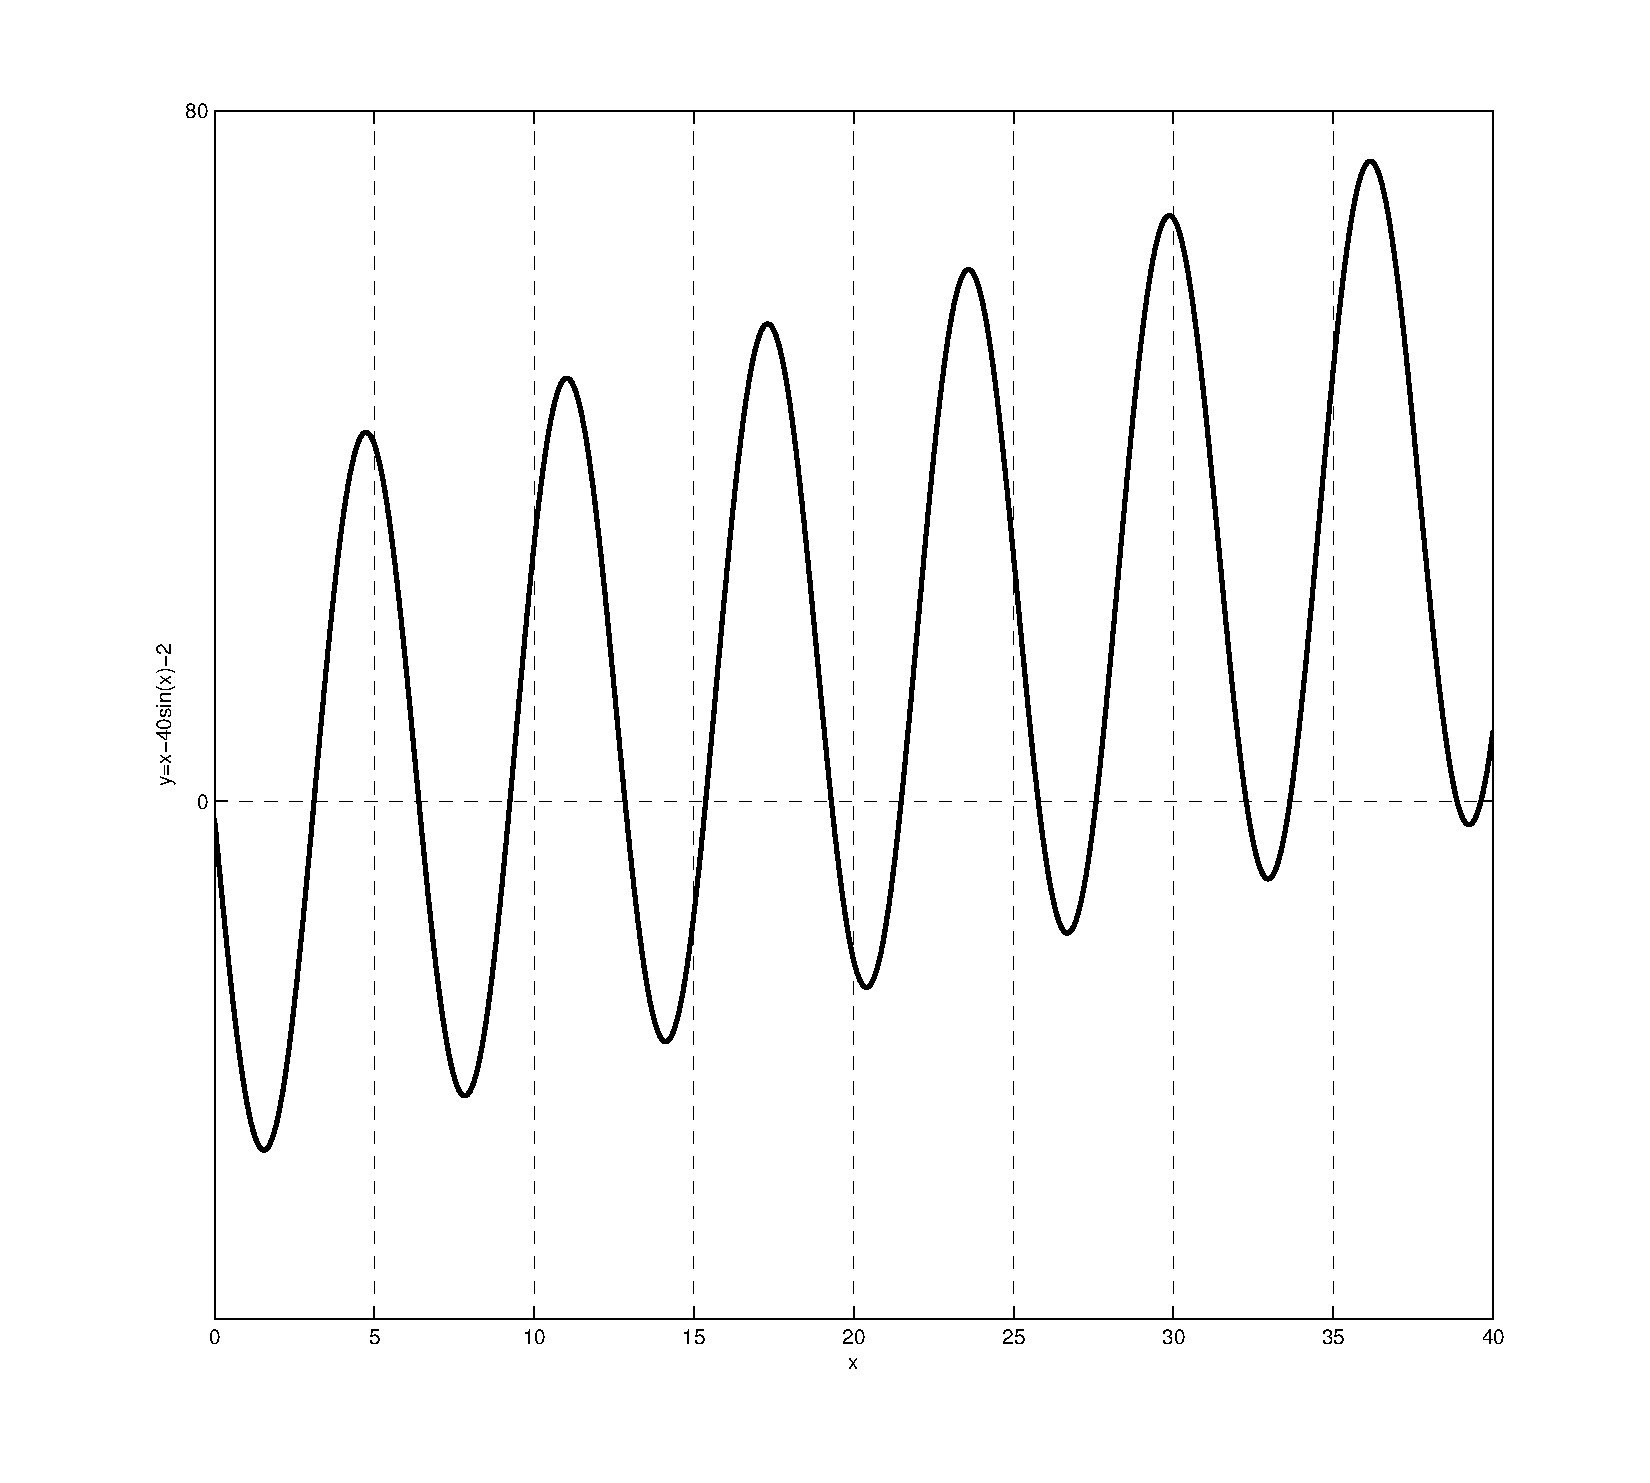
\includegraphics[width=12cm]{kepler.pdf}
	\caption{Ejemplo de ecuación de Kepler para $a=40$ y $b=2$. An Example of Kepler's equation is taking $a=40$ and $b=2$.}
	\label{fig:kepler}
\end{figure}
\begin{paracol}{2}
\paragraph*{Métodos iterativos} 
Todos los métodos que se describen en este capítulo, se basan en procedimientos iterativos. La idea es estimar un valor inicial para la raíz $r_0$, y a partir de él ir refinando paso a paso la solución, de modo que el resultado se acerque cada vez más al valor real de la raíz. Cada nueva aproximación a la raíz se obtiene a partir de las aproximaciones anteriores.
\switchcolumn
\paragraph*{Iterative methods} This chapter solely focuses on iterative techniques. These methods begin with an initial guess for the root, denoted as $r_0$, and then gradually refine the solution through a series of iterative steps. With each step, the solution gets closer and closer to the actual value of the root. The successive approximations of the root are carried out based on the previous ones. 
\end{paracol}
\begin{align*}
r_0\ \ \  \rightarrow \  \ r_1  \ \ \rightarrow \ \ r_2 \ \ \rightarrow \cdots \rightarrow \ \ r_k \ \rightarrow \cdots\\
\vert f(r_0)\vert \ge \vert f(r_1)\vert \ge \vert f(r_2)\vert \ge \cdots \ge \vert f(r_k)\vert \ge \cdots
\end{align*}
\begin{paracol}{2}
El proceso que lleva de una solución aproximada a la siguiente se conoce con el nombre de \emph{iteración}. Lo habitual es que en cada iteración se realicen las mismas operaciones matemáticas una y otra vez. 

El proceso se detiene cuando la solución alcanzada se estima lo suficientemente próxima a la solución real como para darla por buena. Para ello, se suele establecer un valor (\emph{tolerancia}) que actúa como criterio de convergencia. De este modo, las iteraciones se repiten hasta que se llega a un valor $r_n$ 	que cumple,
\begin{equation*}
\vert f(r_n) \vert \leq \text(tol)
\end{equation*}

Se dice entonces que el algoritmo empleado para obtener la raíz ha convergido en \emph{n} iteraciones. Por otro lado, es importante señalar que los algoritmos para el cálculo de raíces de una función no siempre convergen. Hay veces en que no es posible aproximarse cada vez más al valor de la raíz bien por la naturaleza de la función o bien por que el algoritmo no es adecuado para obtenerla.
\switchcolumn

Going from one approximate solution to the next is called \emph{iteration}. Usually, the same mathematical operations are repeated in each iteration.

The iterative process comes to a halt when the obtained solution is considered to be close enough to the actual solution to be considered a good approximation. Typically, a value is set as a convergence criterion, known as tolerance. The iterations continue until a value $r_n$ is obtained that satisfies the criterion.
\begin{equation*}
\vert f(r_n) \vert \leq \text(tol)
\end{equation*}

The algorithm used to obtain the root is then said to have converged in \emph{n} iterations. On the other hand, it is important to note that algorithms for calculating the root of a function do not always converge. Sometimes it is not possible to get closer and closer to the value of the root either because of the nature of the function or because the algorithm is not suitable for obtaining it.

\end{paracol}
\begin{paracol}{2}
\paragraph*{Búsqueda local.} Una función puede tener cualquier número de raíces, incluso infinitas, basta pensar por ejemplo en funciones trigonométricas como $\cos(x)$. Una característica importante de los métodos descritos en este capítulo es que solo son capaces de aproximar una raíz. La raíz de la función a la que el método converge depende de el valor inicial $r_0$ con el que se comienza la búsqueda iterativa\footnote{En ocasiones, como veremos más adelante no se suministra al algoritmo un valor inicial, sino un intervalo en el que buscar la raíz}. Por ello reciben el nombre de métodos locales. Si queremos encontrar varias (o todas) las raíces de una determinada función, es preciso emplear el método para cada una de las raíces por separado, cambiando cada vez el punto de partida.
\switchcolumn

\paragraph*{Local search}. A function can have any number of roots, even infinite ones, just think for example of trigonometric functions such as $\cos(x)$. An important feature of the methods described in this chapter is that they are only able to approximate one root. The root of the function to which the method converges depends on the initial value $r_0$ with which the iterative search is started \footnote{Sometimes, as we will see later on, the algorithm is not given an initial value, but an interval in which to search for the root}. This is why they are called local methods. If we want to find several (or all) the roots of a given function, it is necessary to use the method on each of the roots separately, changing the starting point each time.
\end{paracol}

\begin{paracol}{2}
\section{Metodos iterativos locales}
\subsection{Método de la bisección}
\paragraph*{Teorema de Bolzano.}
\begin{quote}
Si una funcion $f(x)$, continua en el intervalo $[a, b]$, cambia de signo en los extremos del intervalo: $f(a)\cdot f(b) \le 0$, debe tener una raíz en el intervalo [a, b]. (figura: \ref{fig:bolzano}) 
\end{quote}

\switchcolumn
\section{Local iterative methods}
\subsection{Bisection Method}
\paragraph*{Bolzano's theorem}
\begin{quote}
    Let $f(x)$ be a continuous function defined in an interval $[a, b]$. Then, if $f(a)\cdot f(b)<0$
(therefore,$f(a)<0$ and $f(b)>0$ or $f(a)>0$ and $f(b)<0$), there exists at least a point inside the interval $c \in [a,b]$ such that $f(c)=0$. (figure: \ref{fig:bolzano})
\end{quote}
\end{paracol}

\begin{figure}[h]
\centering
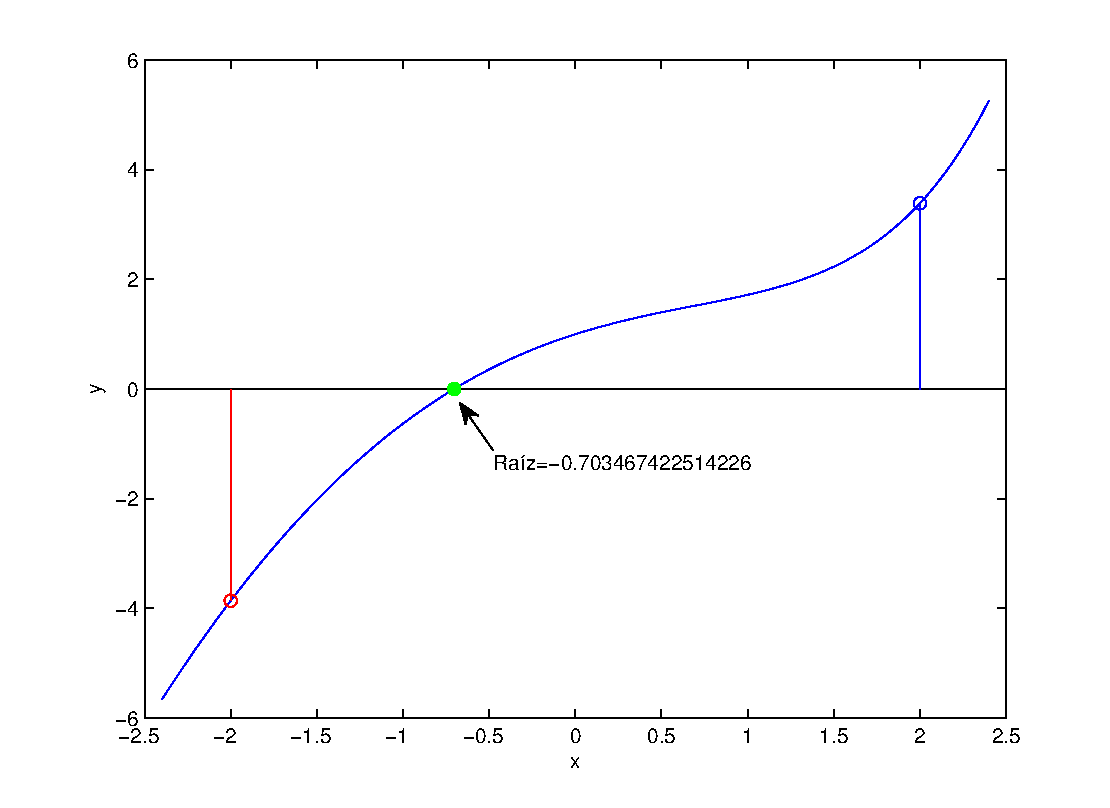
\includegraphics[width=14cm]{bolzano.pdf}
\caption{Ilustración del teorema de Bolzano}
\label{fig:bolzano}
\end{figure}

El conocido teorema de Bolzano, suministra el método más sencillo de aproximar la raíz de una función: Se parte de un intervalo inicial en el que se cumpla el teorema; y se va acotando sucesivamente el intervalo que contiene la raíz, reduciéndolo a la mitad en cada iteración, de forma que en cada nuevo intervalo se cumpla siempre el teorema de Bolzano.

\begin{figure}[h]
\centering
\begin{tikzpicture}
%\usetikzlibrary{shapes.geometric}
\path (5,0) node(a) [rectangle,draw=blue, very thick,align=center,rounded corners]{Partimos de $[a,b]$\\ con\\ $f(a)\cdot f(b)<0$}
(5,-2) node(b)[rectangle,draw=blue, thick,rounded corners]{Calculamos $c=\frac{a+b}{2}, f(c)$}
(5,-4) node(c)[diamond,aspect=3,draw=red,thick]{es $\vert f(c) \vert \le \text{tol}$?}
(9,-4) node(d)[rectangle,draw=blue,align=center,very thick, rounded corners]{convergencia:\\ terminar}
(5,-6) node(e)[diamond,aspect=3,draw=red,thick]{es $f(a)\cdot f(c) < 0$?}
(9.5,-6) node(f)[rectangle,draw=blue,thick,rounded corners,align=center]{$b=c$\\$f(b)=f(c)$}
(5,-8) node(g)[rectangle,draw=blue,thick,rounded corners,align=center]{$a=c$\\$f(a)=f(c)$};
\draw[blue,-latex](a.south)--(b);
\draw[blue,-latex](b.south)--(c);
\draw[blue,-latex](c.east)--(d);
\draw (7.5,-4)node[above]{Sí};
\draw[blue,-latex](c.south)--(e);
\draw (5,-5)node[right]{No};
\draw[blue,-latex](e.east)--(f);
\draw (8,-6)node[above]{Sí};
\draw[blue,-latex](e.south)--(g);
\draw (5,-7.2)node[right]{No};
\draw[blue,-latex](g.south)|-(2,-9)|-(b);
\draw[blue,-latex](f.east)-|(11,-2)--(b);
\end{tikzpicture}
\caption{Diagrama de flujo del método de la bisección}
\label{fig:dfbisec}
\end{figure}
En la figura \ref{fig:dfbisec} se muestra un diagrama de flujo correspondiente al método de la bisección. El punto de partida es un intervalo $[a,b]$ en el que se cumple el teorema de Bolzano, y que contiene por tanto al menos una raíz. Es interesante hacer notar que el teorema de Bolzano se cumple siempre que la función sea continua en el intervalo $[a,b]$ y existan un número impar de raíces. Por esto es importante realizar cuidadosamente la elección del intervalo $[a,b]$, si hay más de una raíz, el algoritmo puede no converger.

 Una vez que se tiene el intervalo se calcula el punto medio $c$. A continuación se compara el valor que toma la función en $c$, es decir $f(c)$ con la tolerancia. Si el valor es menor que ésta, el algoritmo ha encontrado un valor aproximado de la raíz con la tolerancia requerida, con lo que $c$ es la raíz y no hace falta seguir buscando. Si por el contrario, $f(c)$ está por encima de la tolerancia requerida, comparamos su signo con el que toma la función en uno cualquiera de los extremos del intervalo, En el diagrama de flujo se ha elegido el extremo $a$, pero el algoritmo funcionaría igualmente si eligiéramos $b$. Si el signo de $f(c)$ coincide con el que toma la función en el extremo del intervalo elegido, $c$ sustituye al extremo, (hacemos $a=c$ y $f(a)=f(c)$) si por el contrario el signo es distinto, hacemos que $c$ sustituya al otro extremo del intervalo. (hacemos $b=c$ y $f(b)=f(c)$). Este proceso se repetirá hasta que se cumpla que $f(c)\le \text{tol}$ 

El proceso se muestra gráficamente en la figura \ref{fig:bisec}, para un caso particular. Se trata de obtener la raíz de la función mostrada en la figura \ref{fig:bolzano}, $f(x)=e^x-x^2$. esta función tiene una única raíz: $r\approx -0.7035$. Para iniciar el algoritmo se ha elegido un intervalo $[a=-2,b=2]$. La figura \ref{fig:bisec}, muestra tres iteraciones sucesivas,y la solución final, que se obtiene al cabo de ocho iteraciones en éste ejemplo, para el que se a empleado una tolerancia $tol=0.01$. En la secuencia de gráficas se puede observar también la evolución del intervalo de búsqueda, $[-2, 2]\rightarrow [-2, 0] \rightarrow [-1, 0] \rightarrow [-1, -0.5] \cdots$; así como el cambio alternativo del límite derecho o izquierdo, para asegurar que la raíz queda siempre dentro de los sucesivos intervalos de búsqueda obtenidos. 
\begin{figure}
\centering
\subfigure[intervalo inicial]{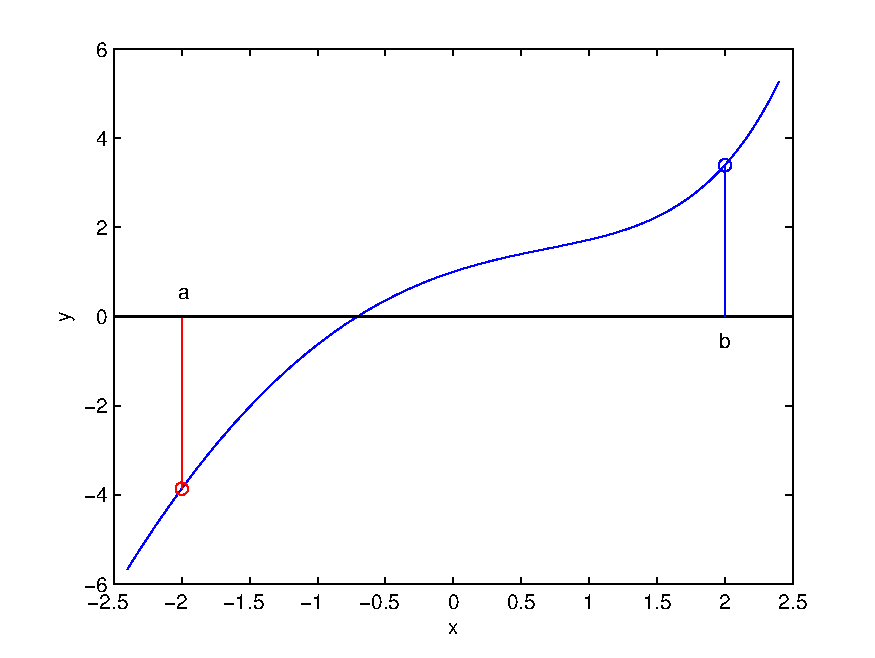
\includegraphics[width=7cm]{rint0.pdf}} \qquad
\subfigure[iteracion 1]{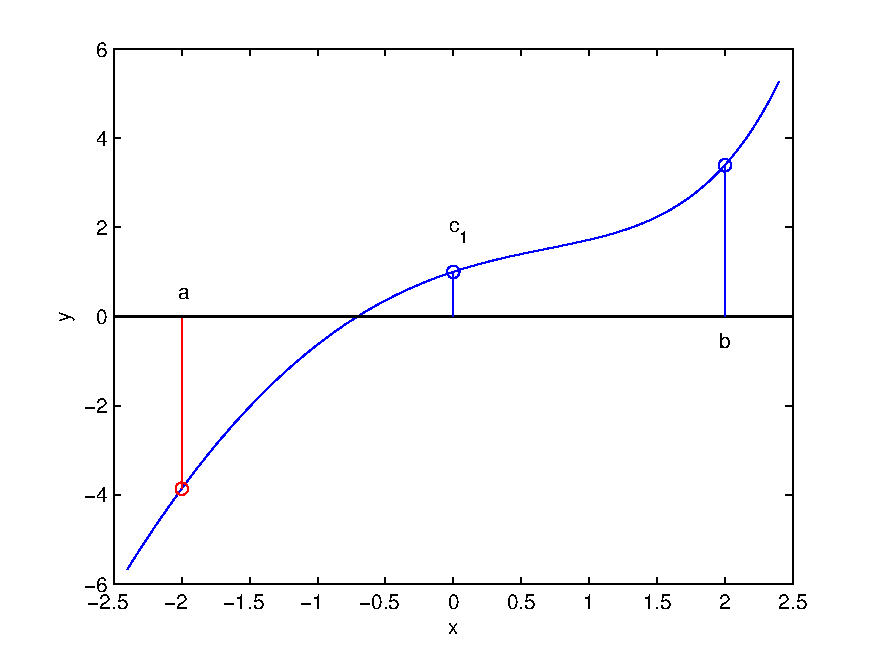
\includegraphics[width=7cm]{rint1.pdf}}\\
\subfigure[iteracion 2]{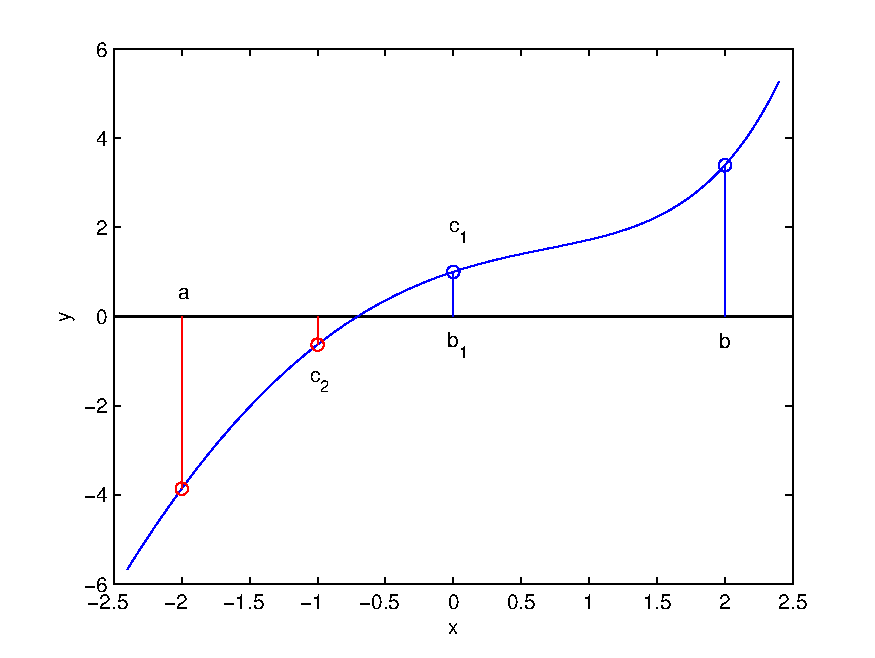
\includegraphics[width=7cm]{rint2.pdf}}\qquad
\subfigure[iteracion 3]{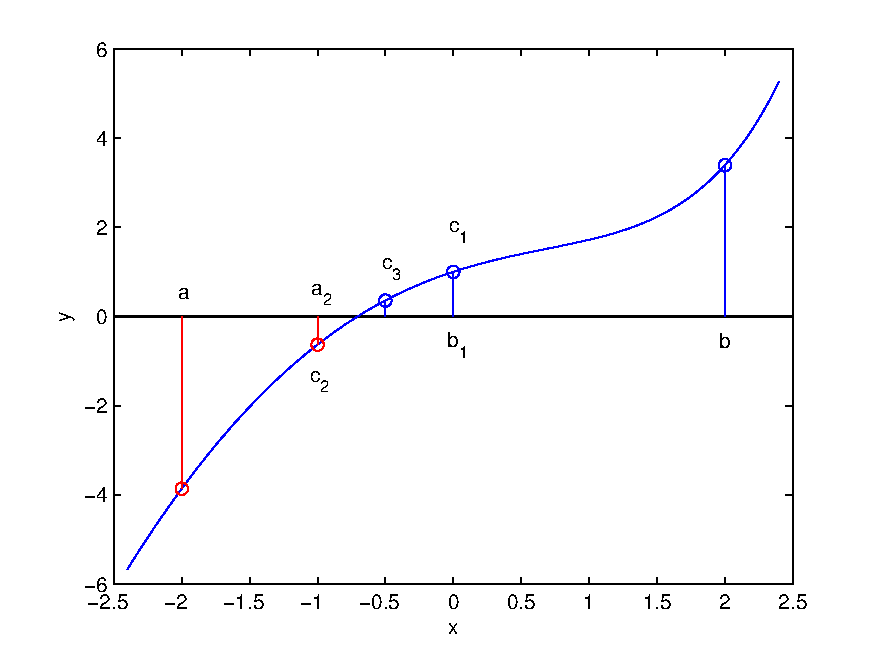
\includegraphics[width=7cm]{rint3.pdf}}\\
\subfigure[iteracion 6: raíz alcanzada]{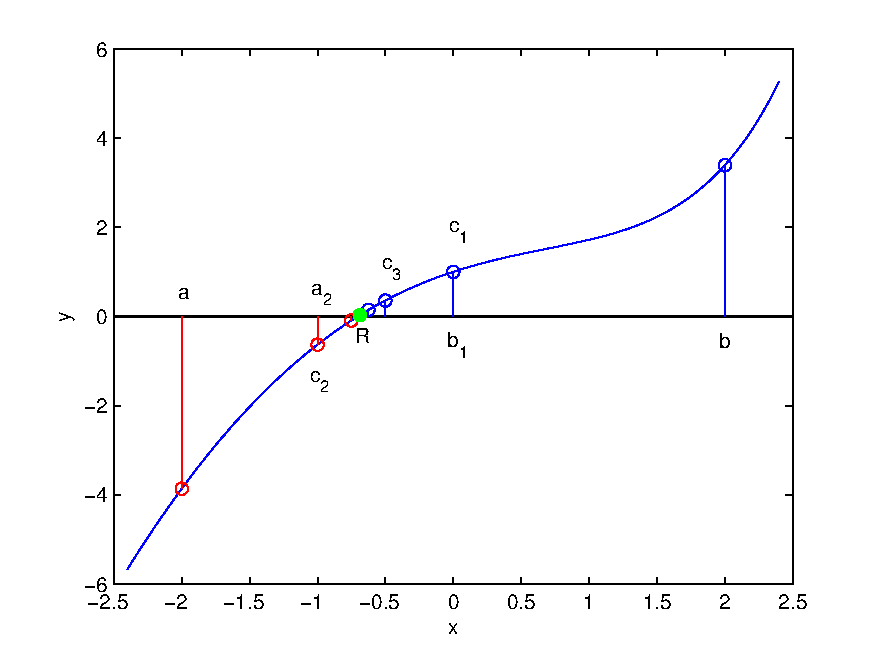
\includegraphics[width=7cm]{rint4.pdf}}

\caption{proceso de obtención de la raíz de una función por el método de la bisección }
\label{fig:bisec}
\end{figure}

\subsection{Método de interpolación lineal o (\emph{Regula falsi})}
Este método supone una mejora del anterior ya que, en general,  converge más rápidamente. La idea es modificar el modo en que calculamos el punto $c$. En el caso del método de la bisección el criterio consistía en ir tomando en cada iteración el punto medio del intervalo que contiene la raíz. El método de interpolación lineal, elige como punto $c$ el punto de corte con el eje x, de la recta que pasa por los puntos $\left(a,f(a)\right)$ y $\left(b,f(b)\right)$. Es decir la recta que corta a la función $f(x)$ en ambos límites del intevalo que contiene a la raíz buscada. La recta que pasa por ambos puntos puede construirse a partir de ellos como,
\begin{equation*}
y=\frac{f(a)-f(b)}{a-b}\cdot(x-b)+f(b)
\end{equation*}
el punto de corte con el eje $x$, que será el valor que tomaremos para $c$, se obtiene cuando $y=0$,
\begin{equation*}
0=\frac{f(a)-f(b)}{a-b}\cdot(x-b)+f(b)
\end{equation*}

y despejando $c\equiv x$ en la ecuación anterior obtenemos,
\begin{equation*}
c=b-\frac{f(b)}{f(b)-f(a)}\cdot(b-a)
\end{equation*}

La figura \ref{fig:regulaf} muestra  gráficamente la posición del punto $c$ obtenido mediante el método de interpolación. 

\begin{figure}[h]
\centering
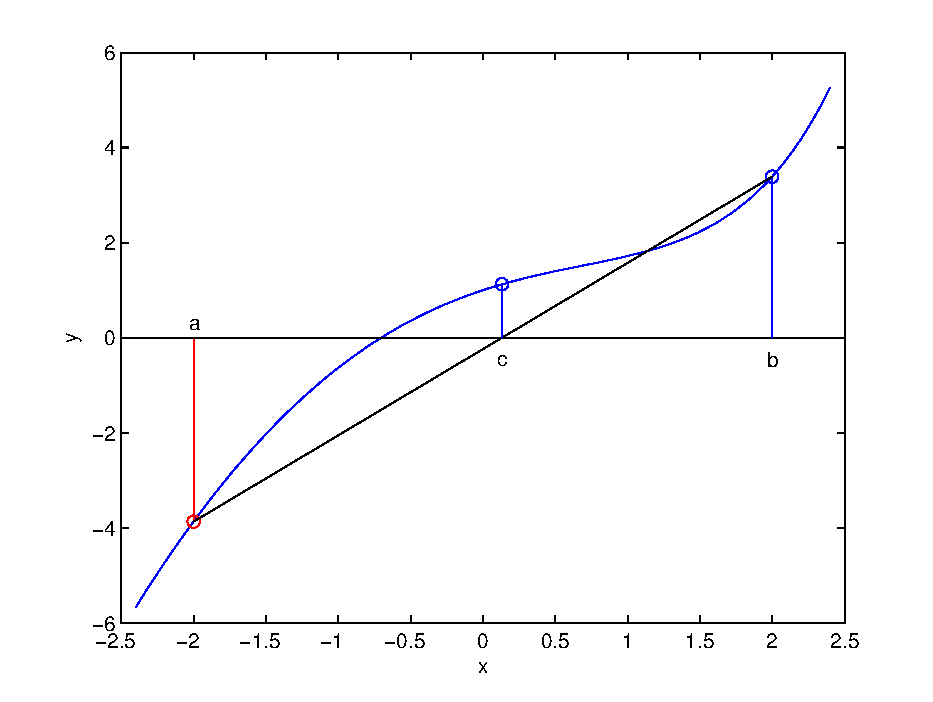
\includegraphics[width=14cm]{rinter00.pdf}

\caption{Obtención de la recta que une los extremos de un intervalo $[a,b]$  que contiene una raíz de la función}
\label{fig:regulaf}
\end{figure}

Por lo demás, el procedimiento es el mismo que en el caso del método de la bisección. Se empieza con un intervalo $[a,b]$ que  contenga una raíz, se obtiene el punto $c$ por el procedimiento descrito y se intercambia $c$ con el extremo del intervalo cuya imagen $f(a)$ o $f(b)$ tenga el mismo signo que $f(c)$ el procedimiento se repite iterativamente hasta que f(c) sea menor que el valor de tolerancia preestablecido. 

\begin{figure}[h]
\centering
\begin{tikzpicture}
%\usetikzlibrary{shapes.geometric}
\path (5,0) node(a) [rectangle,draw=blue, very thick,align=center,rounded corners]{Partimos de $[a,b]$\\ con\\ $f(a)\cdot f(b)<0$}
(5,-2) node(b)[rectangle,draw=blue, thick,rounded corners,align=center]{Calculamos\\ $c=b-\frac{f(b)}{f(b)-f(a)}\cdot(b-a), f(c)$}
(5,-4) node(c)[diamond,aspect=3,draw=red,thick]{es $\vert f(c) \vert \le \text{tol}$?}
(9,-4) node(d)[rectangle,draw=blue,align=center,very thick, rounded corners]{convergencia:\\ terminar}
(5,-6) node(e)[diamond,aspect=3,draw=red,thick]{es $f(a)\cdot f(c) < 0$?}
(9.5,-6) node(f)[rectangle,draw=blue,thick,rounded corners,align=center]{$b=c$\\$f(b)=f(c)$}
(5,-8) node(g)[rectangle,draw=blue,thick,rounded corners,align=center]{$a=c$\\$f(a)=f(c)$};
\draw[blue,-latex](a.south)--(b);
\draw[blue,-latex](b.south)--(c);
\draw[blue,-latex](c.east)--(d);
\draw (7.5,-4)node[above]{Sí};
\draw[blue,-latex](c.south)--(e);
\draw (5,-5)node[right]{No};
\draw[blue,-latex](e.east)--(f);
\draw (8,-6)node[above]{Sí};
\draw[blue,-latex](e.south)--(g);
\draw (5,-7.2)node[right]{No};
\draw[blue,-latex](g.south)|-(2,-9)|-(b);
\draw[blue,-latex](f.east)-|(11,-2)--(b);
\end{tikzpicture}
\caption{Diagrama de flujo del método de interpolación lineal}
\label{fig:regula}
\end{figure}

En la figura \ref{fig:regula} se muestra el diagrama de flujo para el método de interpolación lineal. Como puede verse, es idéntico al de la bisección excepto en el paso en que se obtiene el valor de $c$, donde se ha sustituido el cálculo del punto medio del intervalo de búsqueda, por el cálculo del punto de corte con el eje de abscisas  de la recta que une los extremos del intervalo.

La figura \ref{fig:iterr2} Muestra gráficamente el proceso iterativo seguido para obtener la raíz de una función en un intervalo mediante el método de interpolación lineal. Se ha empleado la misma función y el mismo intervalo inicial que en el caso de la bisección. 

Es fácil ver, sin embargo, que los puntos intermedios que obtiene el algoritmo hasta converger a la raíz son distintos. De hecho, el algoritmo emplea ahora tan solo siete iteraciones para obtener la raíz, empleando el mismo valor para la tolerancia, 0.01, que se empleó en el método de la bisección.

Una observación final, se ha dicho al principio que éste método supone una mejora al método anterior de la bisección. Esto no siempre es cierto. El método de la bisección tiene una tasa de convergencia constante, cada iteración divide el espacio de búsqueda por la mitad. Sin embargo la convergencia del método de interpolación  lineal depende de la función $f(x)$ y de la posición relativa de los puntos iniciales $(a, f(a))$  y $(b, f(b))$ con respecto al la raíz. Por esto no es siempre cierto que converja más rápido que el método de  la bisección. Por otro lado, el cálculo de los sucesivos valores del punto $c$, requiere más operaciones aritméticas en el método de interpolación, con lo que cada iteración resulta más lenta que en el caso de la bisección.
\begin{figure}
\centering
\subfigure[intervalo inicial]{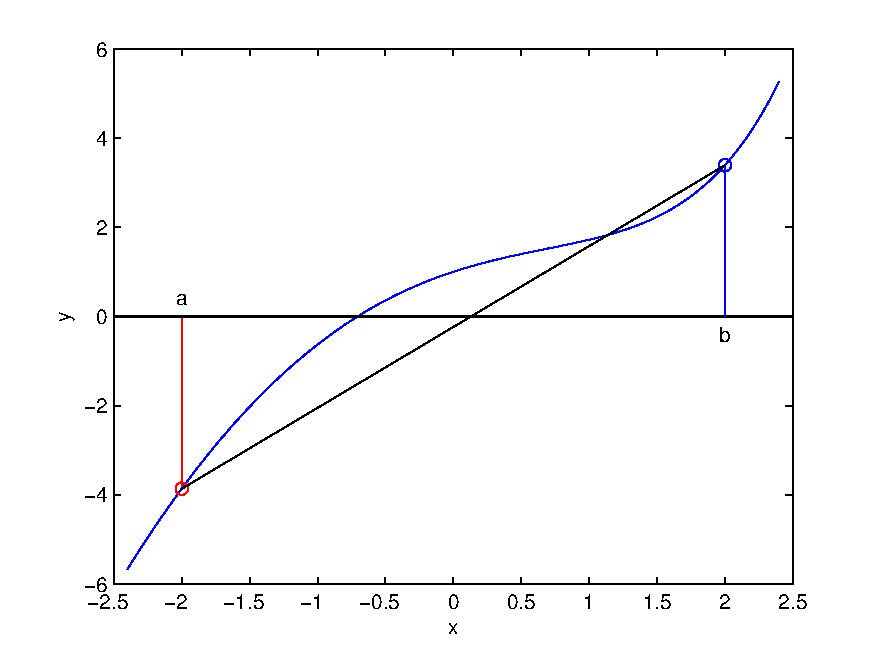
\includegraphics[width=7cm]{rinter0.pdf}} \qquad
\subfigure[iteracion 1]{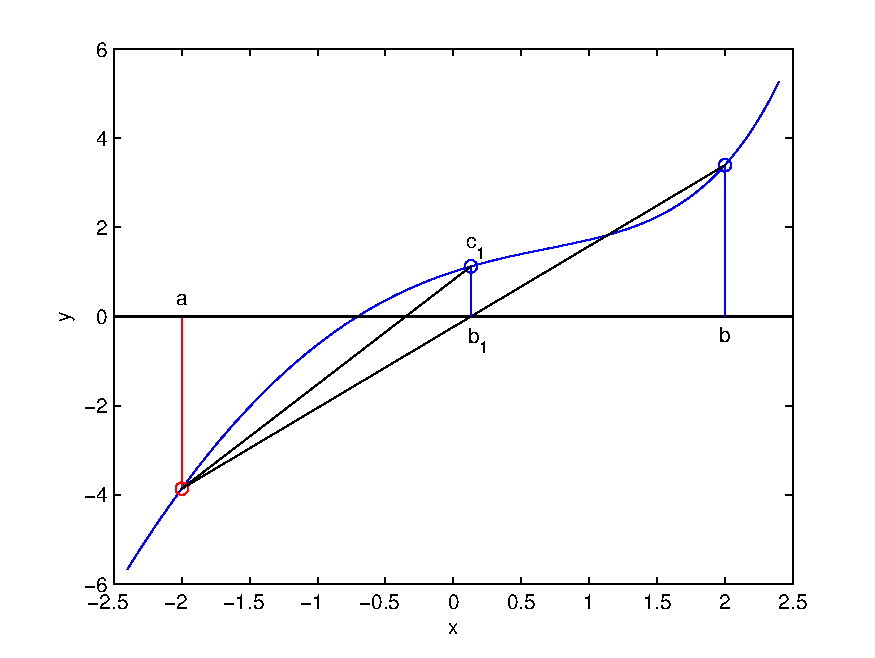
\includegraphics[width=7cm]{rinter1.pdf}}\\
\subfigure[iteracion 2]{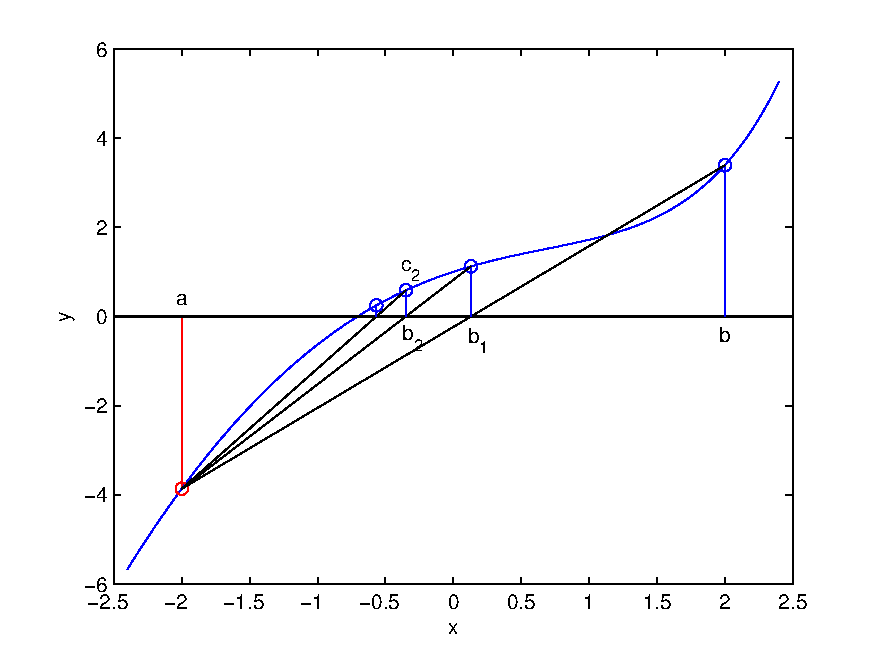
\includegraphics[width=7cm]{rinter2.pdf}}\qquad
\subfigure[iteracion 3]{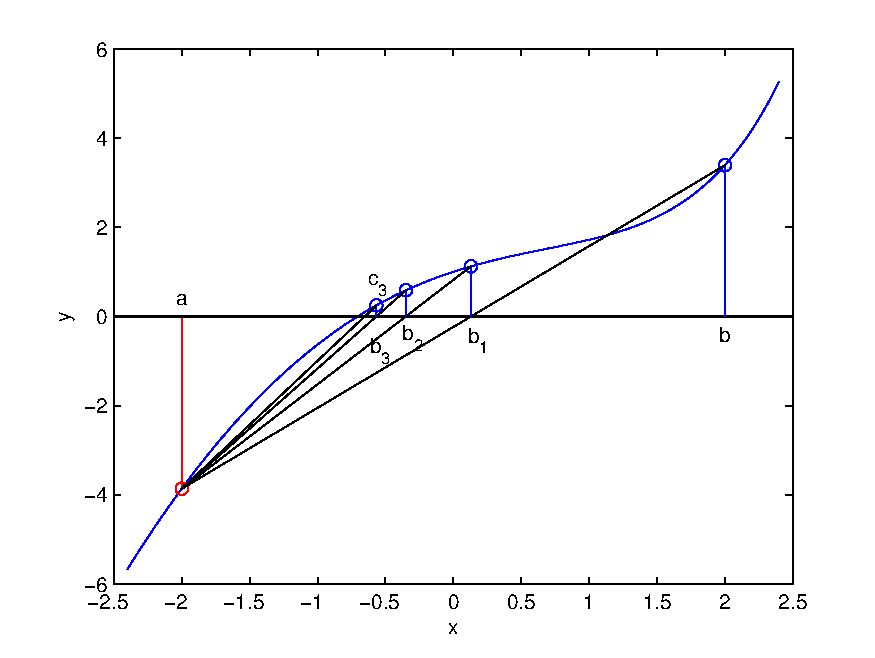
\includegraphics[width=7cm]{rinter3.pdf}}\\
\subfigure[iteracion 6: raíz alcanzada]{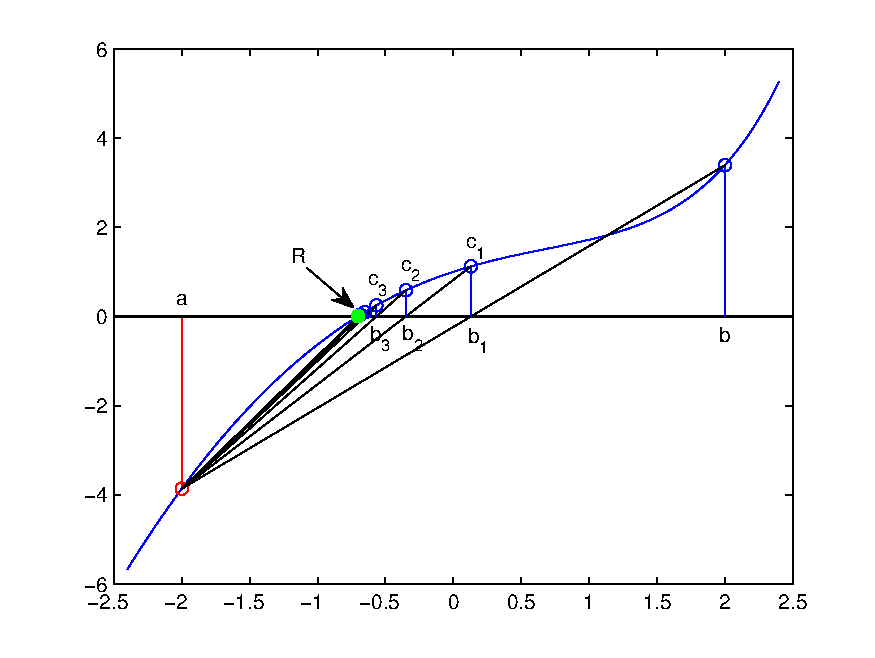
\includegraphics[width=7cm]{rinter4.pdf}}

\caption{Proceso de obtención de la raíz de una función por el método de interpolación lineal}
\label{fig:iterr2}
\end{figure}

\subsection{Método de Newton-Raphson}
El método de Newton se basa en la expansión de una función $f(x)$ en serie de Taylor en el entorno de un punto $x_0$,
\begin{equation*}
f(x)\approx f(x_0)+f'(x_0)(x-x_0)+\frac{1}{2}f''(x_0)(x-x_0)^2+\cdots+\frac{1}{n!}f^{(n)}(x_0)(x-x_0)^n+\cdots
\end{equation*}
 Pertenece a una familia de métodos ampliamente empleados en cálculo numérico. La idea en el caso del método de Newton es aproximar la función para la que se desea obtener la raíz, mediante el primer término de la serie de Taylor. Es decir aproximar localmente $f(x)$, en el entorno de $x_0$ por la recta,
\begin{equation*}
 f(x_0)+f'(x_0)(x-x_0)
\end{equation*}
Esta recta, es precisamente la recta tangente a la curva $f(x)$ en el punto $x_0$ (figura \ref{fig:newton1})
\begin{figure}[h]
\centering
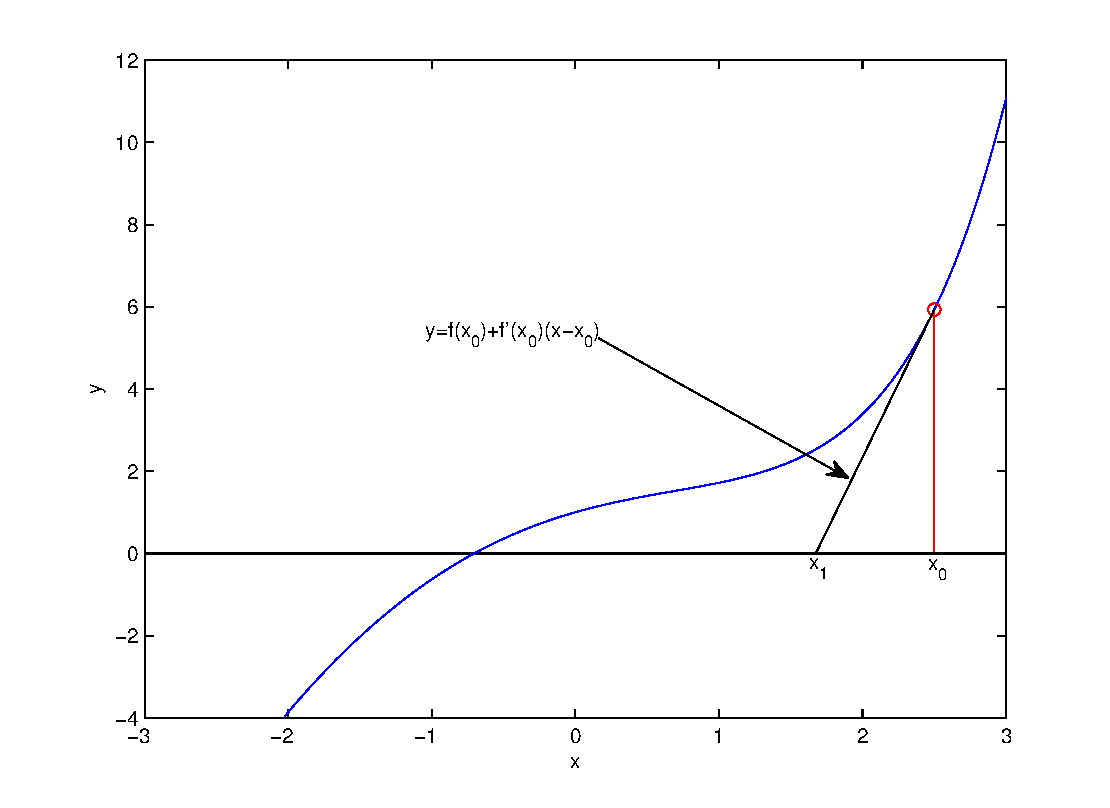
\includegraphics[width=14cm]{newt0.pdf}[h]
\caption{Recta tangente a la función $f(x)$ en el punto $x_0$}
\label{fig:newton1}
\end{figure}

El método consiste en obtener el corte de esta recta tangente con el eje de abscisas,
\begin{equation*}
0= f(x_0)+f'(x_0)(x-x_0)
\end{equation*}

y despejando x,

\begin{equation*}
x=x_0-\frac{f(x_0)}{f'(x_0)}
\end{equation*}

A continuación se evalúa la función en el punto obtenido $x\rightarrow f(x)$. Como en los métodos anteriores, se compara el valor de $f(x)$ con una cierta tolerancia preestablecida. Si es menor, el valor de $x$ se toma como raíz de la función. Si no, se vuelve aplicar el algoritmo, empleando ahora el valor de x que acabamos de obtener como punto de partida. Cada cálculo constituye una nueva iteración y los sucesivos valores obtenidos para $x$, convergen a la raíz,

\begin{equation*}
x_0\rightarrow x_1=x_0-\frac{f(x_0)}{f'(x_0)}\rightarrow x_2=x_1-\frac{f(x_1)}{f'(x_1)}\rightarrow  \cdots \rightarrow x_n=x_{n-1}-\frac{f(x_{n-1})}{f'(x_{n-1})}\rightarrow \cdots
\end{equation*}

La figura \ref{fig:newton} muestra un diagrama de flujo correspondiente al método de Newton. Si se compara con los diagramas de flujo de los algoritmos anteriores, el algoritmo de Newton resulta algo más simple de implementar. Sin embargo es preciso evaluar en cada iteración el valor de la función y el de su derivada. 

El cálculo de la derivada, es el punto débil de este algoritmo, ya que para valores $x_0$ próximos a un mínimo o máximo local obtendremos valores de la derivada próximos a cero, lo que puede causar un error de desbordamiento al calcular el punto de corte de la recta tangente con el eje de abscisas o hacer que el algoritmo converja a una raíz alejada del punto inicial de búsqueda.
 
\begin{figure}[h]
\centering
\begin{tikzpicture}
%\usetikzlibrary{shapes.geometric}
\path (5,0) node(a) [rectangle,draw=blue, very thick,align=center,rounded corners]{Partimos de un punto inicial $x_0$}
(5,-2) node(b)[rectangle,draw=blue, thick,rounded corners,align=center]{Calculamos\\ $x=x_0-\frac{f(x_0)}{f'(x_0)}, f(x)$}
(5,-4) node(c)[diamond,aspect=3,draw=red,thick]{es $\vert f(x) \vert \le \text{tol}$?}
(9,-4) node(d)[rectangle,draw=blue,align=center,very thick, rounded corners]{convergencia:\\ terminar}
(5,-6) node(g)[rectangle,draw=blue,thick,rounded corners,align=center]{$x_0=x$};
\draw[blue,-latex](a.south)--(b);
\draw[blue,-latex](b.south)--(c);
\draw[blue,-latex](c.east)--(d);
\draw (7.5,-4)node[above]{Sí};
\draw[blue,-latex](c.south)--(g);
\draw (5,-5)node[right]{No};
\draw[blue,-latex](g.south)|-(2,-7)|-(b);

\end{tikzpicture}
\caption{Diagrama de flujo del método de Newton-Raphson}
\label{fig:newton}
\end{figure}

La figura \ref{fig:newton2} muestra un ejemplo de obtención de la raíz de una función mediante el método de Newton. El método es más rápido que los dos anteriores, es decir, partiendo de una distancia comparable a la raíz, es el que converge en menos iteraciones. 

En el ejemplo de la figura se ha obtenido la raíz para la misma función que en los ejemplos del método de la bisección e interpolación lineal. Se ha empezado sin embargo en un punto más alejado de la raíz, para que pueda observarse mejor en la figura la evolución del algoritmo. En cada uno de los gráficos que componen la figura pueden observarse  los pasos del algoritmo: dado el punto  $x_i$, se calcula  la recta tangente a la función $f(x)$ en el punto y se obtiene un nuevo punto $x_{i+1}$,  como el corte de dicha recta tangente con el eje de abscisas.

En este ejemplo el algoritmo converge en las cinco iteraciones que se muestran en la figura, para la misma tolerancia empleada en los métodos anteriores, $tol=0.01$. El punto de inicio empleado fue $x_0=2.5$, por tanto esta fuera del intervalo $[-2, 2]$ y más alejado de la raíz que en el caso de los métodos anteriores.   

\begin{figure}
\centering
\subfigure[intervalo inicial]{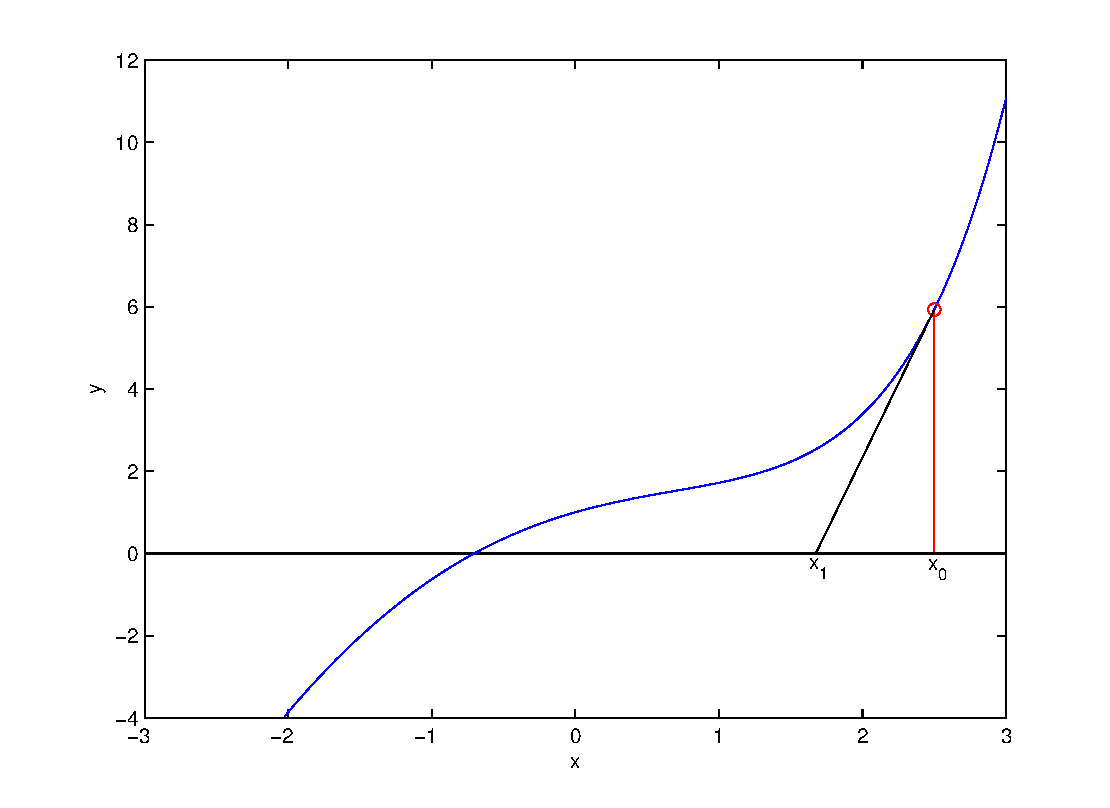
\includegraphics[width=7cm]{newt01.pdf}} \qquad
\subfigure[iteracion 1]{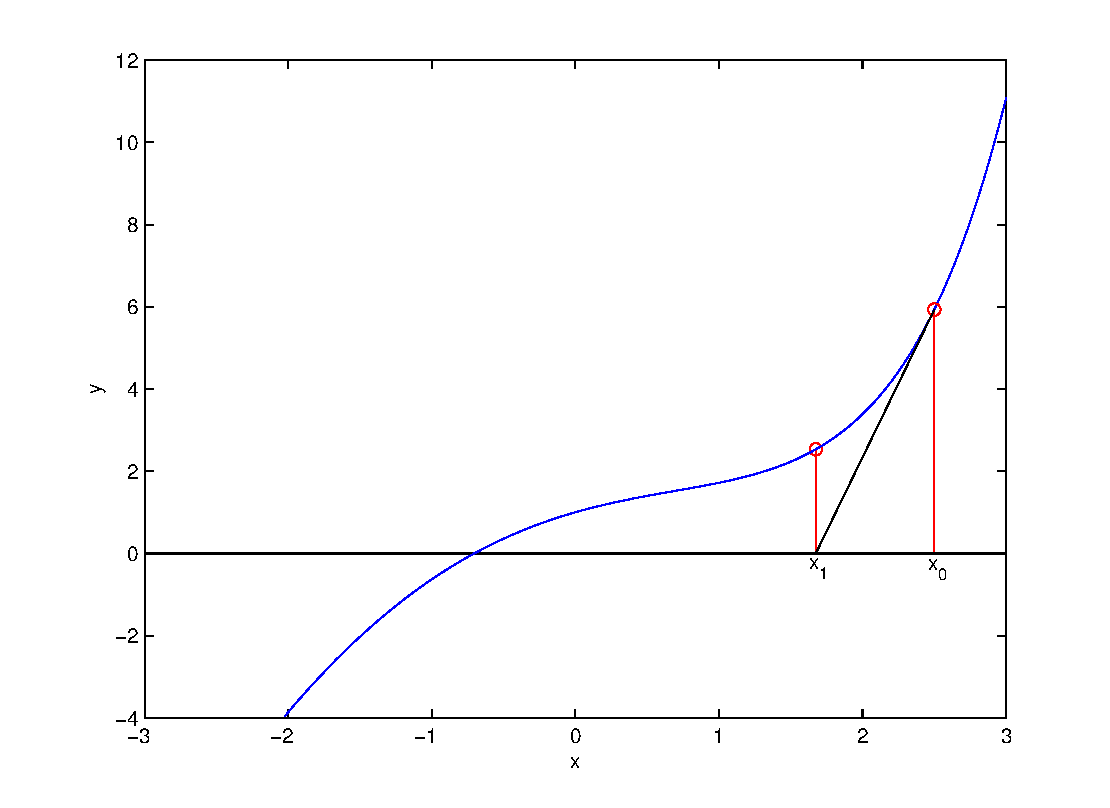
\includegraphics[width=7cm]{newt02.pdf}}\\
\subfigure[iteracion 2]{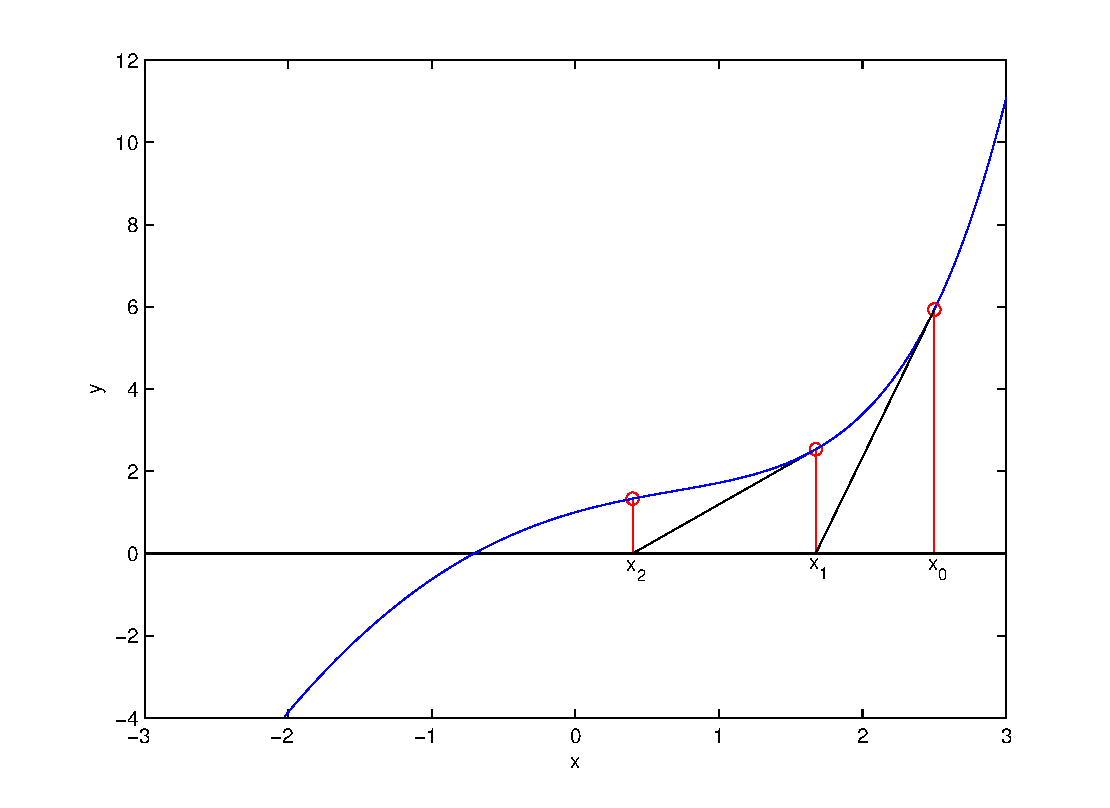
\includegraphics[width=7cm]{newt1.pdf}}\qquad
\subfigure[iteracion 3]{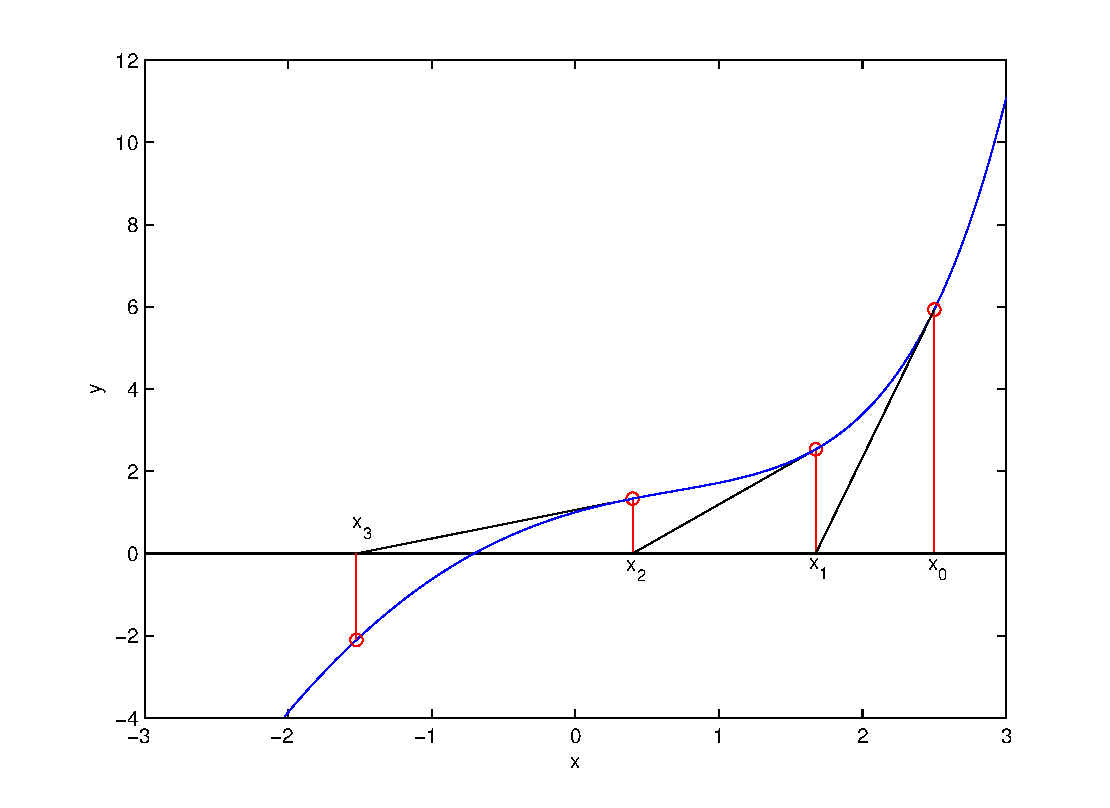
\includegraphics[width=7cm]{newt2.pdf}}\\
\subfigure[iteracion 4]{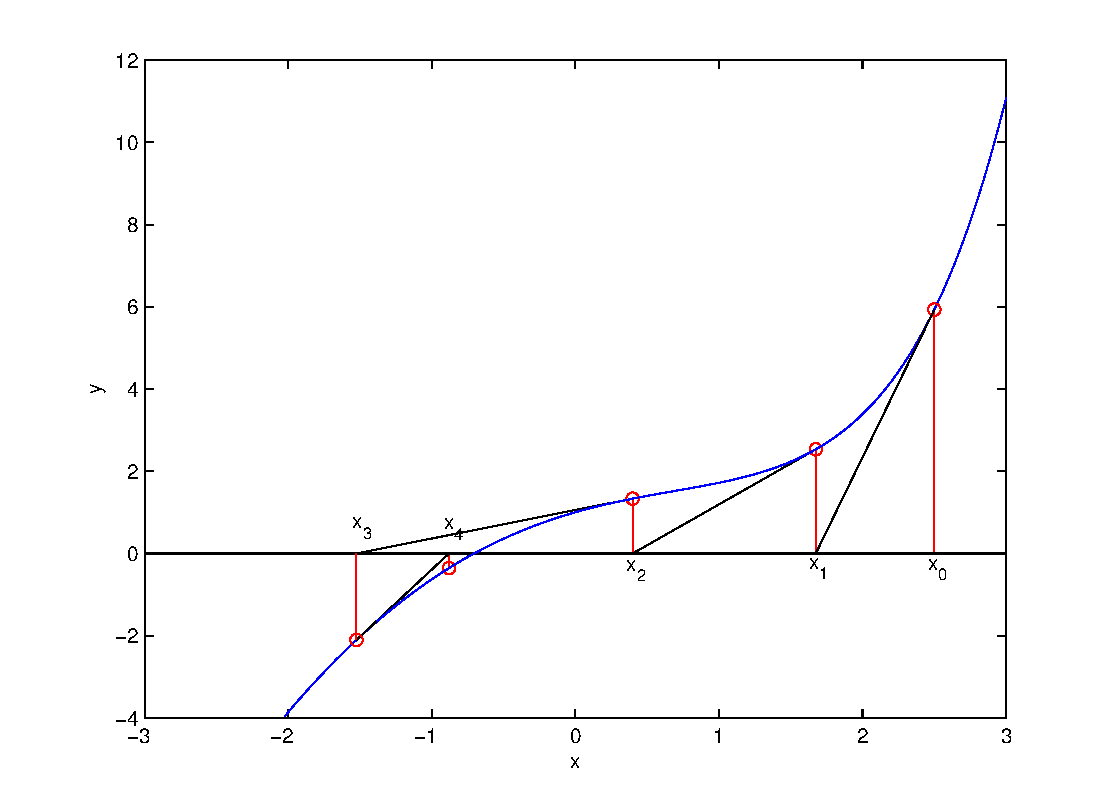
\includegraphics[width=7cm]{newt3.pdf}}\qquad
\subfigure[iteracion 5: raíz de la función]{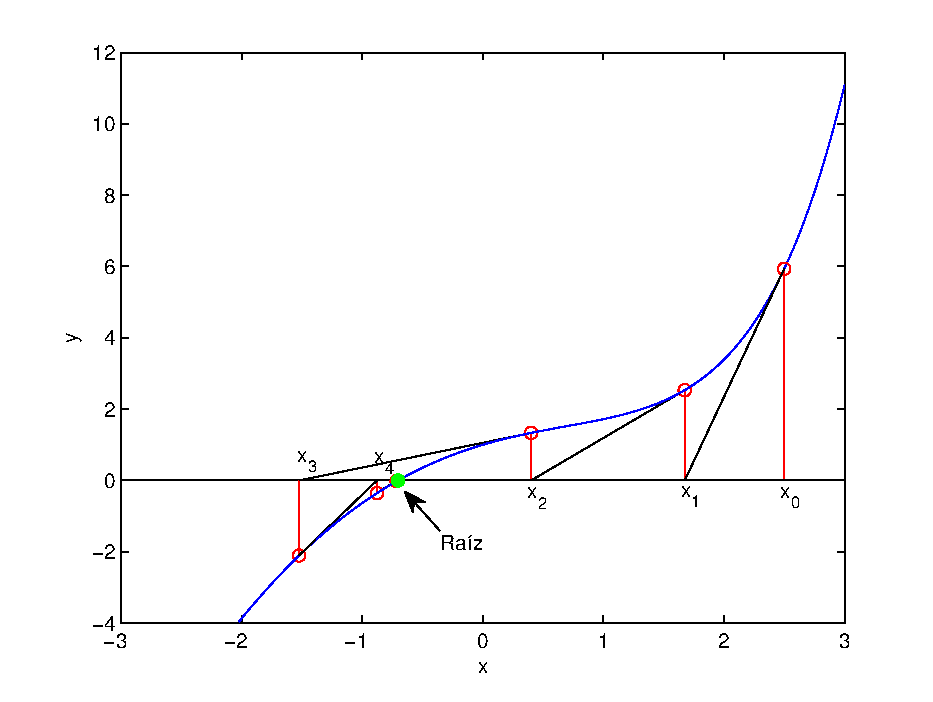
\includegraphics[width=7cm]{newt4.pdf}}

\caption{Proceso de obtención de la raíz de una función por el método de Newton}
\label{fig:newton2}
\end{figure}
\subsection{Método de la secante}
El método de la secante podría considerarse una variante del método de newton en el que se sustituye la recta tangente al punto $x0$ por la recta secante que une dos puntos obtenidos en iteraciones sucesivas. La idea es \emph{aproximar} la derivada a la función $f$ en el punto $x_n$ por la pendiente de una recta secante, es decir de una recta que corta a la función en dos puntos, 
\begin{equation*}
f'(x_n)\approx \frac{f(x_n)-f(x_{n-1})}{x_n-x_{n-1}}
\end{equation*}

Las sucesivas aproximaciones a la raíz de la función se obtienen de modo similar a las del método de Newton, simplemente sustituyendo la derivada de la función por su valor aproximado,

\begin{equation*}
x_{n+1}=x_n-\frac{f(x_n)}{f'(x_n)}\approx x_n-\frac{(x_n-x_{n-1})\cdot f(x_n)}{f(x_n)-f(x_{n-1})}
\end{equation*}

Para iniciar el algoritmo, es preciso emplear en este caso dos puntos iniciales. La figura \ref{fig:secante} muestra un ejemplo.

\begin{figure}[h]
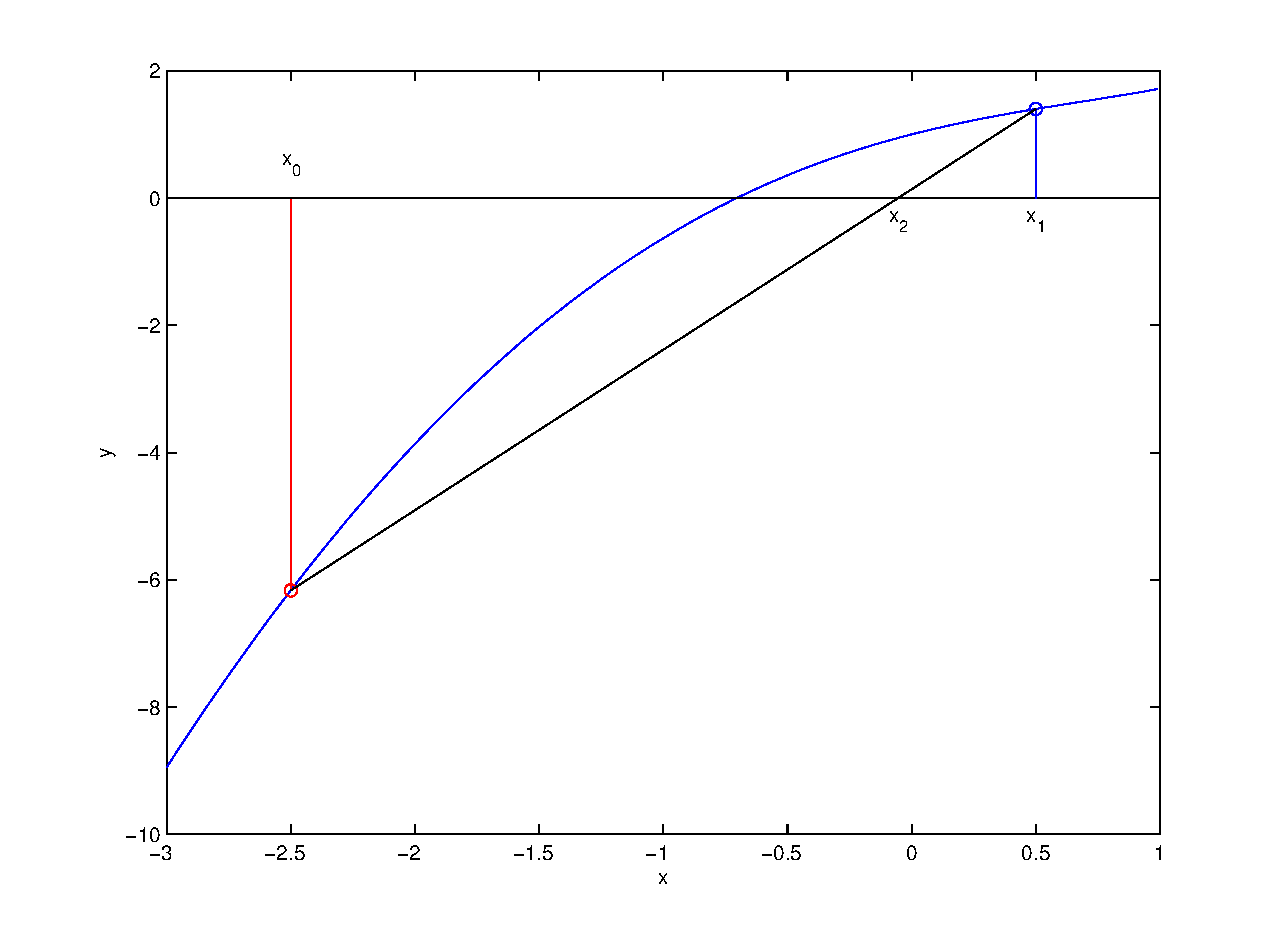
\includegraphics[width=14cm]{secante0.pdf}
\caption{Recta secante a la  función $f(x)$ en los puntos $x_0$ y $x_1$}
\label{fig:secante}
\end{figure}

El método podría en este punto confundirse con el de interpolación, sin embargo tiene dos diferencias importantes: En primer lugar, la elección de los dos puntos iniciales $x_0$ e $x_1$, no tienen por qué formar un intervalo que contenga a la raíz. Es decir, podrían estar ambos situados al mismo lado de la raíz. En segundo lugar, los puntos obtenidos se van sustituyendo por orden, de manera que la nueva recta secante se construye siempre a partir de los dos últimos puntos obtenidos, sin prestar atención a que el valor de la raíz esté contenido entre ellos. (No se comparan los signos de la función en los puntos para ver cual se sustituye, como en el caso del método de interpolación). 

La figura \ref{fig:secante2} muestra un diagrama de flujo para el método de la secante. El diagrama es básicamente el mismo que el empleado para el método de Newton. Las dos diferencias fundamentales son, que ahora en lugar de evaluar la función y la derivada en cada iteración, se calcula  el valor del punto de corte de la recta que pasa por los dos últimos puntos obtenidos (es decir, empleamos una recta secante, que corta a la curva en dos puntos, en lugar de emplear una recta tangente). 

Además es preciso actualizar, en cada iteración, el valor de los dos últimos puntos obtenidos: el más antiguo se desecha, el punto recién obtenido sustituye al anterior y éste al obtenido dos iteraciones antes. 

\begin{figure}[h]
\centering
\begin{tikzpicture}
%\usetikzlibrary{shapes.geometric}
\path (5,0) node(a) [rectangle,draw=blue, very thick,align=center,rounded corners]{Partimos de dos puntos inicial $x_0$, $x_1$}
(5,-2) node(b)[rectangle,draw=blue, thick,rounded corners,align=center]{Calculamos\\ $x=x_1-\frac{(x_1-x_0)\cdot f(x_1)}{f(x_1)-f(x_0)}, f(x)$}
(5,-4) node(c)[diamond,aspect=3,draw=red,thick]{es $\vert f(x) \vert \le \text{tol}$?}
(9,-4) node(d)[rectangle,draw=blue,align=center,very thick, rounded corners]{convergencia:\\ terminar}
(5,-6) node(g)[rectangle,draw=blue,thick,rounded corners,align=center]{$x_0=x_1$\\ $x_1=x$};
\draw[blue,-latex](a.south)--(b);
\draw[blue,-latex](b.south)--(c);
\draw[blue,-latex](c.east)--(d);
\draw (7.5,-4)node[above]{Sí};
\draw[blue,-latex](c.south)--(g);
\draw (5,-5)node[right]{No};
\draw[blue,-latex](g.south)|-(2,-7)|-(b);

\end{tikzpicture}
\caption{Diagrama de flujo del método de la secante}
\label{fig:secante2}
\end{figure}

La figura \ref{fig:secante3} muestra un ejemplo de la obtención de una raíz por el método de la secante. Se ha empleado de nuevo la misma función que en los ejemplos anteriores, tomando como valores iniciales, $x_0=-2.5$ y $x_1=0.5$. La tolerancia se ha fijado en $tol=0.01$ también como en los anteriores algoritmos descritos. En este caso, el algoritmo encuentra la raíz en cinco iteraciones. Cada uno de los gráficos que compone la figura \ref{fig:secante3}, muestra la obtención de un nuevo punto a partir de los dos anteriores. 

En la iteración 2, puede observarse como el nuevo punto se obtiene a partir de dos puntos que están ambos situados a la derecha de la raíz, es decir, no forman un intervalo que contenga a la raíz.  Aquí se pone claramente de manifiesto la diferencia con el método de interpolación lineal. De hecho, com ya se ha dicho, el método de la secante puede iniciarse tomando los dos primeros puntos a uno de los lados de la raíz.

 El método es, en principio, más eficiente que el de la bisección y el de interpolación lineal, y menos eficiente que el de Newton.

La ventaja de este método respecto al de Newton es que evita tener que calcular explícitamente la derivada de la función para la que se quiere calcular la raíz. El algunos casos, la obtención de la forma analítica de dicha derivada puede ser compleja.   

\begin{figure}
\centering
\subfigure[intervalo inicial]{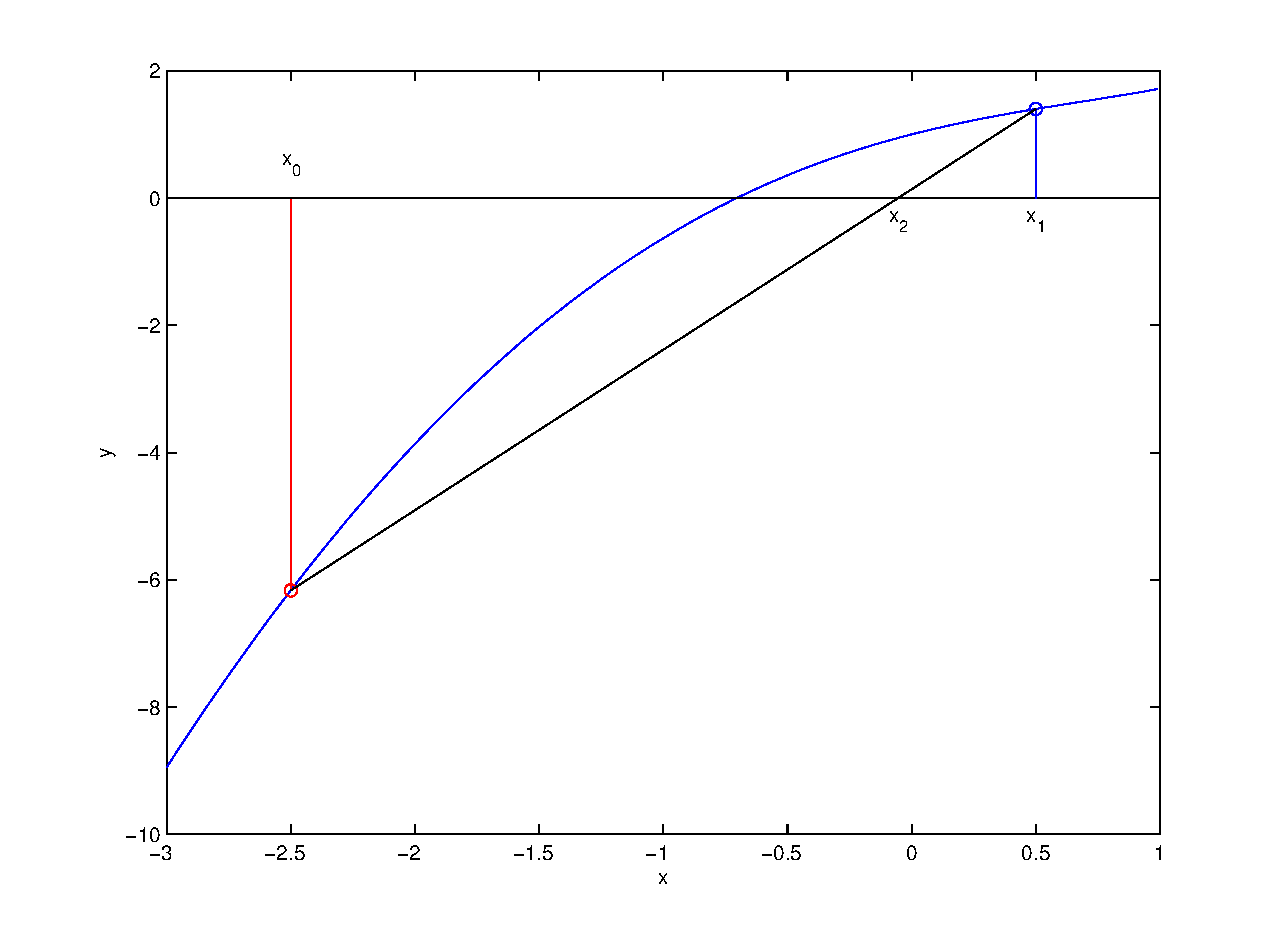
\includegraphics[width=7cm]{secante0.pdf}} \qquad
\subfigure[iteracion 1]{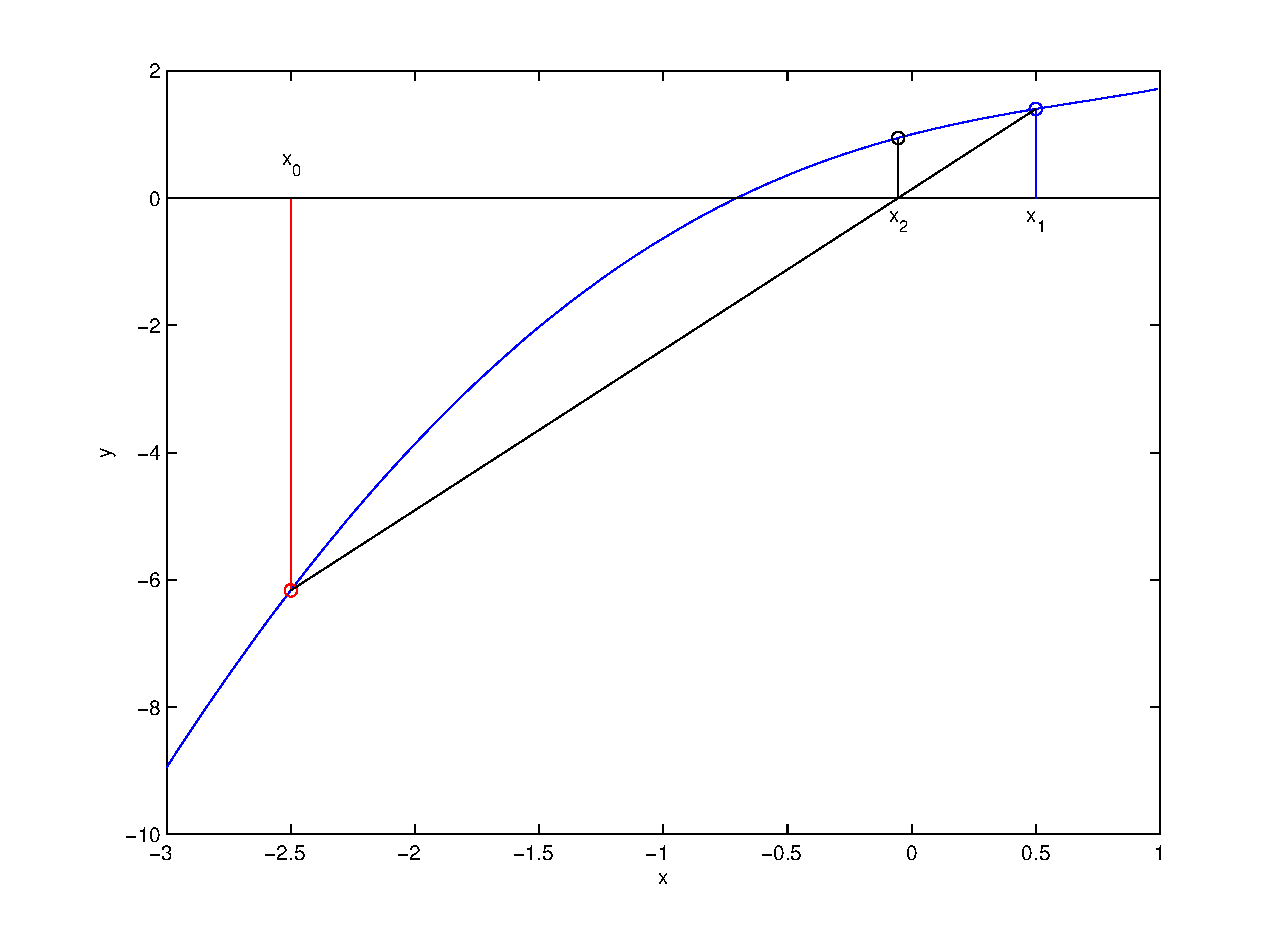
\includegraphics[width=7cm]{secante1.pdf}}\\
\subfigure[iteración 2]{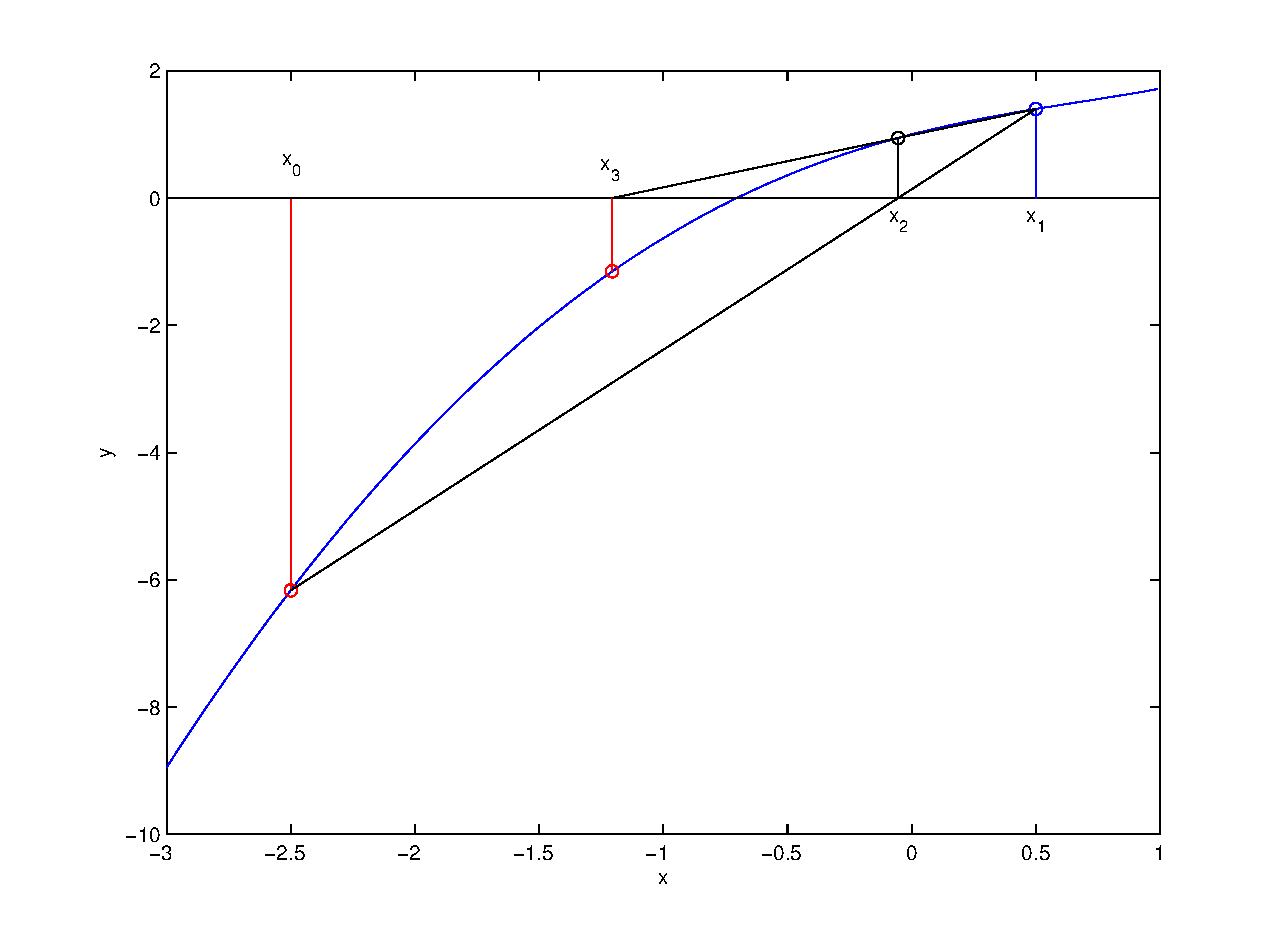
\includegraphics[width=7cm]{secante2.pdf}}\qquad
\subfigure[iteración 3]{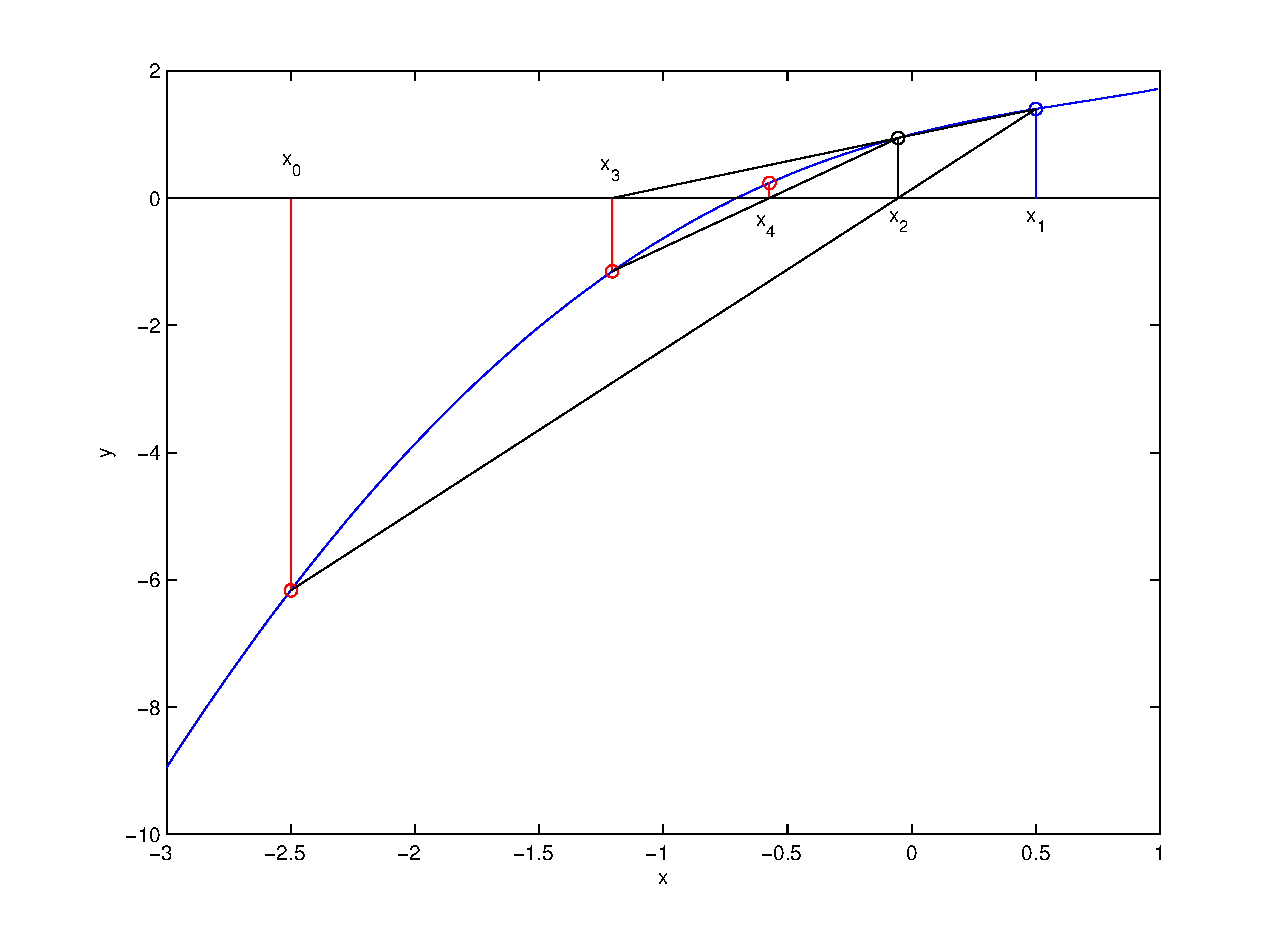
\includegraphics[width=7cm]{secante3.pdf}}\\
\subfigure[iteración 4]{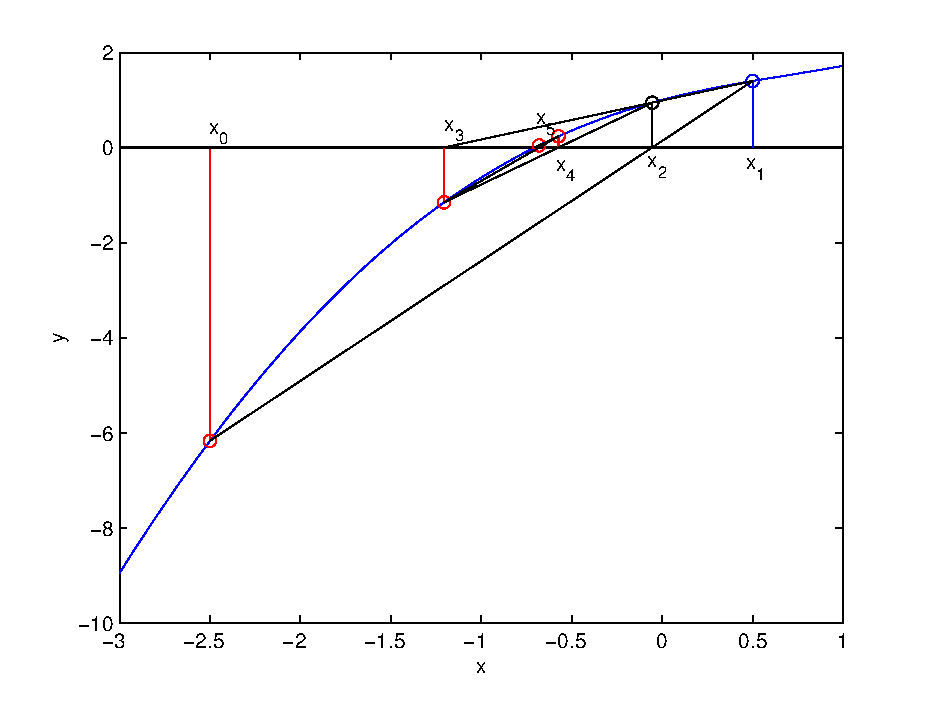
\includegraphics[width=7cm]{secante31.pdf}}\qquad
\subfigure[iteración 5]{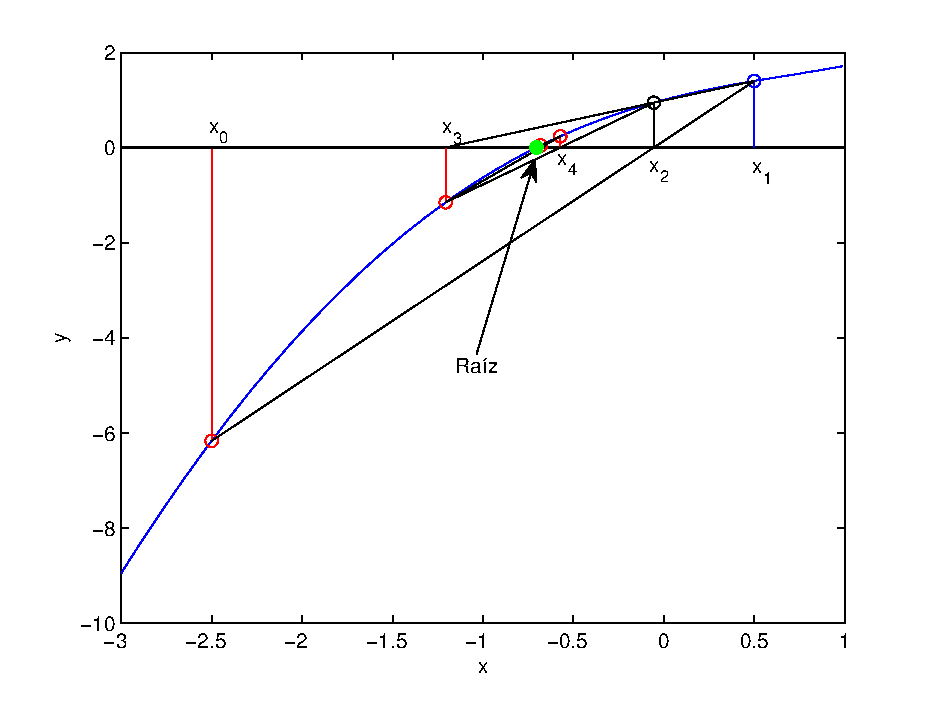
\includegraphics[width=7cm]{secante4.pdf}}

\caption{proceso de obtención de la raíz de una función por el método de la secante}
\label{fig:secante3}
\end{figure}

\subsection{Método de las aproximaciones sucesivas o del punto fijo}\label{pfijo}

El método del punto fijo es, como se verá a lo largo de esta sección, el más sencillo de programar de todos. Desafortunadamente, presenta el problema de que no podemos aplicarlo a todas las funciones. Hay casos en los que el método no converge, con lo que no es posible emplearlo para encontrar la raíz o raíces de una función.
 
\paragraph{Punto fijo de una función.} \index{Punto fijo! de una función}Se dice que un punto $x_f$ es un punto fijo de una función $g(x)$ si se cumple,
\begin{equation*}
g(x_f)=x_f
\end{equation*}

Es decir, la imagen del punto fijo $x_f$ es de nuevo el punto fijo. Así por ejemplo la función,
\begin{equation*}
g(x)=-\sqrt{e^x}
\end{equation*}

Tiene un punto fijo en $x_f=-0.703467$, porque $g(-0.703467)=-0.703467$. La existencia de un punto fijo puede obtenerse gráficamente, representando en un mismo gráfico la función $y=g(x)$ y la recta $y=x$. Si existe un punto de corte entre ambas gráficas, se trata de un punto fijo.  La figura \ref{fig:pfijo0}, muestra gráficamente el punto fijo de la función $g(x)=-\sqrt{e^x}$ del ejemplo anterior.

Una función puede tener uno o más puntos fijos o no tener ninguno. Por ejemplo, la función $y=\sqrt{e^x}$ no tiene ningún punto fijo.


\begin{figure}[h]
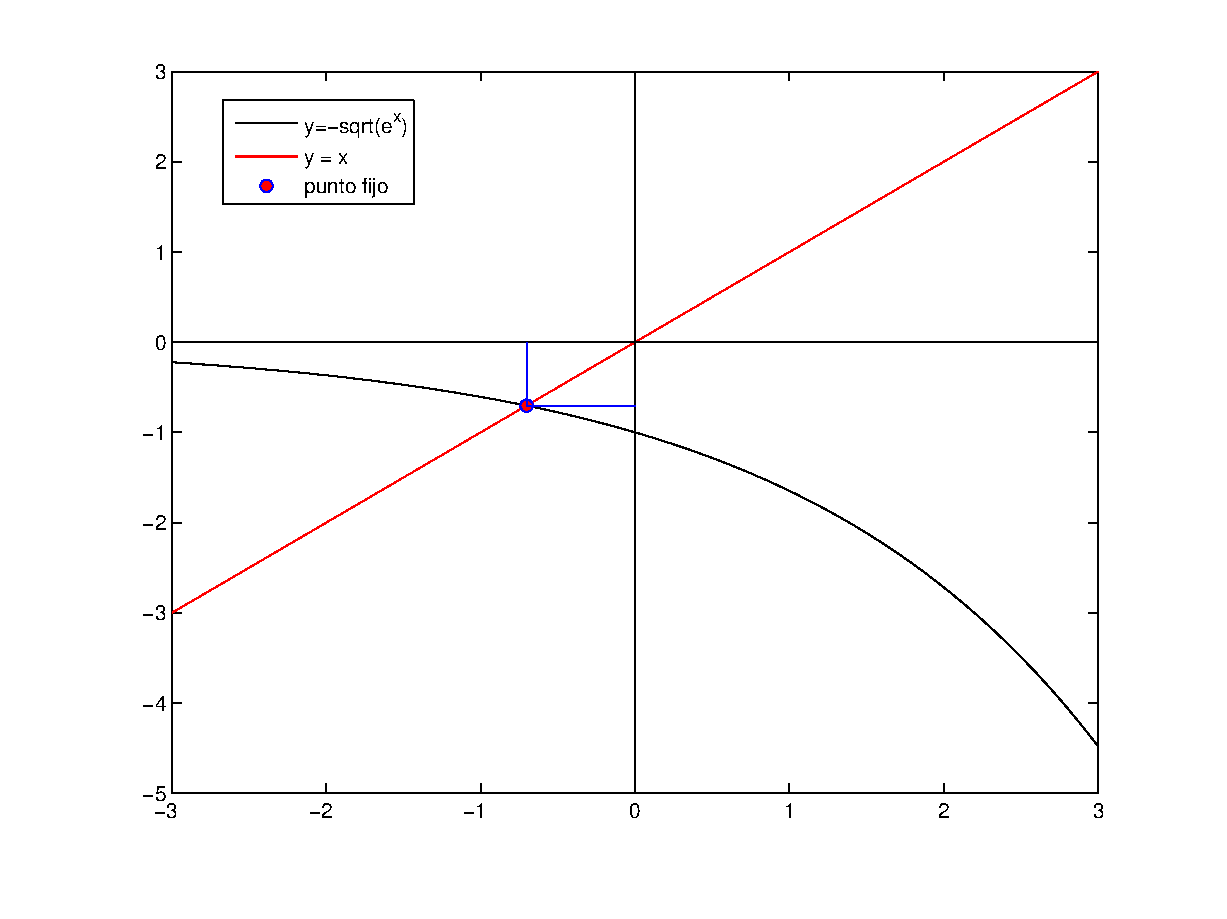
\includegraphics[width=14cm]{pfijo0.eps}
\caption{Obtención gráfica del punto fijo de la función, $g(x)=-\sqrt{e^x}$}
\label{fig:pfijo0}
\end{figure}

\paragraph{Punto fijo atractivo.} \index{Punto fijo! atractivo}Supongamos ahora que, a partir de la función $g(x)$ creamos la siguiente sucesión,
\begin{equation*}
x_{n+1}=g(x_n)
\end{equation*}

Es decir, empezamos tomando un punto inicial $x_0$ y a partir de él vamos obteniendo los siguientes valores de la sucesión como,
\begin{equation*}
x_0\rightarrow x_1=g(x_0)\rightarrow x_2=g(x_1)=g\left(g(x_0)\right) \rightarrow \cdots \rightarrow x_{n+1}=g(x_{n})=g\left( g\left( \cdots\left( g(x_0)\right)\right)\right) \rightarrow \cdots
\end{equation*}
Decimos que un punto fijo $x_f$ de la función $g(x)$ es un punto fijo atractivo si la sucesión $x_{n+1}=g(x_n)$ converge al valor $x_f$, siempre que $x_0$ se tome \emph{suficientemente} cercano a $x_f$. Cómo de cerca tienen que estar $x_0$ y $x_f$ para que la serie converja, es una cuestión delicada. De entrada, es importante descartar que hay funciones que tienen puntos fijos no atractivos, por ejemplo, la función $g(x)=x^2$ tiene dos puntos fijos $x=0$ y $x=1$. El primero es el límite de la sucesión $x_{n+1}=g(x_n)$ para cualquier valor inicial $x_0$ contenido en el intervalo abierto $(-1,  1)$. El punto $x=1$ resulta inalcanzable para cualquier sucesión excepto que el punto de inicio sea él mismo $x_0=x_f=1$.

Hay algunos casos en los que  es posible, para determinadas funciones, saber cuando uno de sus puntos fijos es atractivo,

\paragraph{Teorema de existencia y unicidad del punto fijo.}\index{Punto fijo! Teorema} Dada una función $g(x)$,  continua y diferen-\- ciable en un intervalo $[a, b]$, si se cumple que, $\forall x \in [a, b] \Rightarrow g(x)\in [a,b]$,  entonces $g(x)$ tiene un punto fijo en el intervalo $[a, b]$. 

Si además existe una constante positiva $k < 1$  y se  cumple que  la derivada $\vert g'(x) \vert \leq k, \  \forall x \in (a, b)$, entonces el punto fijo contenido en $[a,b]$ es único. 

Para demostrar la primera parte del teorema, se puede emplear el teorema de Bolzano. Si se cumple que $g(a)=a$ o que  $g(b)=b$, entonces $a$ o $b$ serían el punto fijo. Supongamos que no es así;  entonces tiene que cumplirse que $g(a)>a$ y que $g(b)<b$. Si construimos una función, $f(x)=g(x)-x$ esta función, que es continua por construcción, cumple que $f(a)=g(a)-a>0$ y $f(b)=g(b)-b<0$. Pero entonces, debe existir un punto, $x_f \in [a, b]$ para el cual $f(x_f)=0$ y, por tanto, $f(x_f)=g(x_f)-x_f=0 \Rightarrow g(x_f)=x_f$. Es decir, $x_f$ es un punto fijo de $g(x)$.

La segunda parte del teorema puede demostrarse empleando el teorema de valor medio. Si suponemos  que existen dos puntos fijos distintos $x_{f1} \neq x_{f2}$ en el intervalo $[a,b]$, según el teorema del valor medio, existe un punto $\xi$ comprendido entre $x_{f1}$ y $ x_{f2}$ para el que se cumple,

\begin{equation*}
\frac{g(x_{f1})-g(x_{f2})}{x_{f1}-x_{f2}}=g'(\xi)
\end{equation*}

Por tanto,

\begin{equation*}
\vert g(x_{f1})-g(x_{f2}) \vert =\vert x_{f1}-x_{f2} \vert\cdot \vert g'(\xi) \vert \leq \vert x_{f1}-x_{f2} \vert \cdot k < \vert x_{f1}-x_{f2} \vert 
\end{equation*}

Pero como se trata de puntos fijos $\vert g(x_{f1})-g(x_{f2}) \vert =\vert x_{f1}-x_{f2}\vert $. con lo que llegaríamos al resultado contradictorio, 

 \begin{equation*}
\vert x_{f1}-x_{f2}\vert=\vert g(x_{f1})-g(x_{f2}) \vert  \leq \vert x_{f1}-x_{f2} \vert\cdot k < \vert x_{f1}-x_{f2} \vert 
\end{equation*}

Salvo que, en contra de la hipótesis inicial, se cumpla que  $ x_{f1}=x_{f2}$. En cuyo caso, solo puede existir un único punto fijo en el intervalo $[a, b]$ bajo las condiciones impuestas por el teorema.

\paragraph{Teorema de punto fijo (atractivo).} \footnote{Hay varios teoremas de punto fijo definidos en distintos contextos matemáticos. Aquí se da una versión reducida a funciones $f(x):\mathbb{R} \rightarrow \mathbb{R}$} Dada una función $g(x)$,  continua y diferenciable en un intervalo $[a, b]$, que  cumple que, $\forall x \in [a, b] \Rightarrow g(x)\in [a,b]$ y que  $\vert g'(x) \vert \leq k, \  \forall x \in (a, b)$, con $0<k<1$, entonces se cumple que, para cualquier punto inicial $x_0$, contenido en el intervalo $[a, b]$, la sucesión  $x_{n+1}=g(x_n)$ converge al único punto fijo del intervalo $[a, b]$.

La demostración puede obtenerse de nuevo a partir del teorema del valor medio.  Si lo aplicamos al valor inicial $x_0$ y al punto fijo $x_f$, obtenemos,

\begin{equation*}
\vert g(x_0)-g(x_f) \vert =\vert x_0-x_f \vert \cdot \vert g'(\xi) \vert \leq \vert x_0-x_f \vert \cdot k 
\end{equation*}

Para la siguiente iteración tendremos,

\begin{equation*}
\vert g(x_1)-g(x_f) \vert \leq \vert x_1-x_f \vert \cdot k \leq \vert x_0-x_f \vert \cdot k^2 
\end{equation*}

puesto que,  $x_1=g(x_0)$ y $x_f = g(x_f)$, puesto que $x_f$ es el punto fijo. 

Por simple inducción tendremos que para el término enésimo de la sucesión,

\begin{equation*}
\vert g(x_n)-g(x_f) \vert \leq \vert x_{n-1}-x_f \vert \cdot k \leq \vert x_{n-2}-x_f \vert \cdot k^2 \leq \cdots \leq  \vert x_0-x_f \vert \cdot k^n 
\end{equation*}

Pero
\begin{equation*}
\underset{n\rightarrow \infty}{\text{lim}}k^n=0 \Rightarrow \underset{n\rightarrow \infty}{\text{lim}} \vert x_n-x_f \vert \leq \underset{n\rightarrow \infty}{\text{lim}}\vert x_0-x_f \vert k^n =0
\end{equation*} 

Es decir, la sucesión  $x_{n+1}=g(x_n)$ converge al punto fijo $x_f$.


\paragraph{El método del punto fijo.}\index{Punto fijo! Método} Como ya hemos visto, obtener una raíz de una función $f(x)$, consiste en resolver la ecuación $f(x)=0$. Supongamos que podemos descomponer la función $f(x)$ como la diferencia de dos términos, una función auxiliar, $g(x)$, y la propia variable $x$
\begin{equation*}
f(x)=g(x)-x
\end{equation*}

Encontrar una raíz de $f(x)$ resulta entonces equivalente a buscar un punto fijo de $g(x)$. 

\begin{equation*}
f(x)=0 \rightarrow g(x)-x=0 \rightarrow g(x)=x
\end{equation*}

En general, a partir de una función dada $f(x)$, es posible encontrar distintas funciones $g(x)$ que cumplan que $f(x)=g(x)-x$. No podemos garantizar que cualquiera de las descomposiciones que hagamos nos genere una función $g(x)$ que tenga un punto fijo. 
Además, para funciones que tengan más de una raíz, puede suceder que distintas descomposiciones de la función converjan a distintas raíces.
Si podemos encontrar una que cumpla las condiciones del teorema de punto fijo que acabamos de enunciar, en un entorno de una raíz de $f(x)$, podemos desarrollar un método que obtenga iterativamente los valores de la sucesión   $x_{n+1}=g(x_n)$, a partir de un valor inicial $x_0$.  El resultado se aproximará al punto fijo de $g(x)$, y por tanto a la raíz de $f(x)$ tanto como queramos. Bastará, como   en los métodos anteriores, definir un valor (tolerancia), por debajo del cual consideramos que el valor obtenido es suficientemente próximo a  la raíz como para darlo por válido. 

La figura \ref{fig:pfijo1} muestra un diagrama de flujo del método del punto fijo. 


\begin{figure}[h]
\centering
\begin{tikzpicture}
%\usetikzlibrary{shapes.geometric}
\path (5,0) node(a) [rectangle,draw=blue, very thick,align=center,rounded corners]{Partimos de un punto inicial $x_0$}
(5,-2) node(b)[rectangle,draw=blue, thick,rounded corners,align=center]{Calculamos\\ $x=g(x_0)$}
(5,-4) node(c)[diamond,aspect=3,draw=red,thick]{es $\vert  x-x_0 \vert \le \text{tol}$?}
(9,-4) node(d)[rectangle,draw=blue,align=center,very thick, rounded corners]{convergencia:\\ terminar}
(5,-6) node(g)[rectangle,draw=blue,thick,rounded corners,align=center]{$x_0=x$};
\draw[blue,-latex](a.south)--(b);
\draw[blue,-latex](b.south)--(c);
\draw[blue,-latex](c.east)--(d);
\draw (7.5,-4)node[above]{Sí};
\draw[blue,-latex](c.south)--(g);
\draw (5,-5)node[right]{No};
\draw[blue,-latex](g.south)|-(2,-7)|-(b);

\end{tikzpicture}
\caption{Diagrama de flujo del método del punto fijo. Nótese que la raíz obtenida corresponde a la función $f(x)=g(x)-x$}
\label{fig:pfijo1}
\end{figure}

 La idea es elegir cuidadosamente el punto inicial $x_0$, para asegurar que se encuentra dentro del intervalo de convergencia del punto fijo.  A continuación, calculamos el valor de $g(x_0)$, el resultado será un nuevo valor  $x$ .  Comprobamos la diferencia entre el punto obtenido y el anterior y si es menor que una cierta tolerancia,  consideramos que el método ha convergido, dejamos de iterar, y devolvemos el valor de $x$ obtenido como resultado. Si no, copiamos $x$ en $x_0$ y volvemos a empezar todo el proceso. Es interesante hacer notar que que el algoritmo converge cuando la diferencia entre dos puntos consecutivos es menor que un cierto valor.  De acuerdo con la \emph{condición } de punto fijo $g(x_0)=x_0$, dicha distancia, sería equivalente a la que media entre $f(x_0)=g(x_0)-x_0$, la función para la que queremos obtener la raíz,   y $0$.

Veamos un ejemplo. Supongamos  que queremos calcular por el método del punto fijo la raíz de la  
función $y=e^x-x^2$, que hemos empleado en los ejemplos de los métodos anteriores.

En primer lugar, debemos obtener a partir de ella una nueva función que cumpla que $f(x)=g(x)-x$. Podemos hacerlo de varias maneras despejando una '$x$', de la ecuación $e^x-x^2=0$.  Para ilustrar los distintos casos de convergencia, despejaremos $x$ de tres maneras distintas .

\begin{equation*}
e^x-x^2=0 \Rightarrow \left\{
\begin{aligned}
x&=\pm  \sqrt{e^x}\\
x&= ln(x^2)=2\cdot ln(\vert x \vert)\\
x&=\frac{e^x}{x} 
\end{aligned} 
\right.
\end{equation*}

\begin{figure}[h]
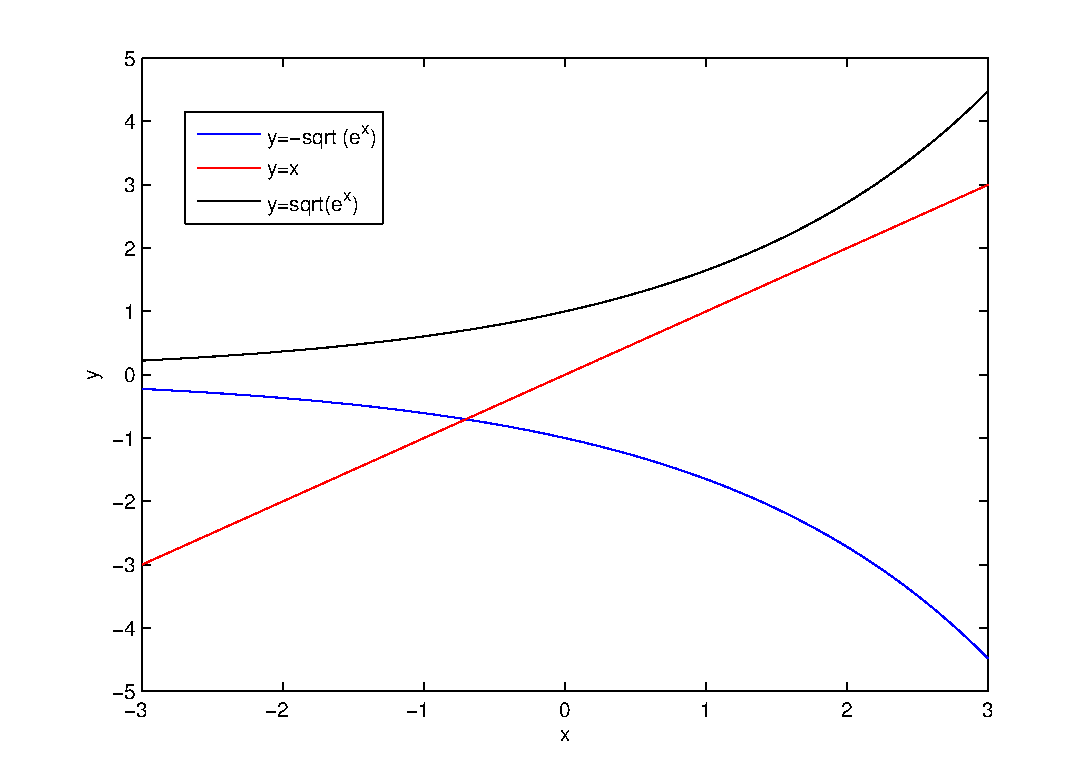
\includegraphics[width=14cm]{pfijo1.pdf}
\caption{$g(x)=\pm \sqrt{e^x}$, Solo la rama negativa tiene un punto fijo.}
\label{fig:pfijo01}
\end{figure}

En nuestro ejemplo hemos obtenido tres formas distintas de \emph{despejar} la variable $x$. La cuestión que surge inmediatamente es, si todas las funciones obtenidas, tienen un punto fijo y, en caso de tenerlo, si es posible alcanzarlo iterativamente.

En el primer caso, $x=\pm \sqrt{e^x}$, obtenemos las dos ramas de la raíz cuadrada. Cada una de ellas constituye a los efectos de nuestro cálculo una función distinta. Si las dibujamos junto a la recta $y=x$ (figura \ref{fig:pfijo01}), observamos que solo la rama negativa la corta. Luego será  esta rama $g(x)=-\sqrt{e^x}$,  la que podremos utilizar para obtener la raíz de la función original por el método del punto fijo. La rama positiva, al no cortar a la recta $y=x$ en ningún punto, es una función que carece de punto fijo.

No es difícil demostrar, que la función $g(x)=-\sqrt{e^x} $ cumple las condiciones del teorema de punto fijo descrito más arriba para el intervalo $(-\infty, 0]$. Luego el algoritmo del punto fijo debería converger para cualquier punto de inicio $x_0$ contenido en dicho intervalo. De hecho, para esta función, el algoritmo converge desde cualquier punto de inicio (Si empezamos en punto positivo, el siguiente punto, $x_1$ será negativo, y por tanto estará dentro del intervalo de convergencia). Esta función es un ejemplo de que el teorema suministra una condición suficiente, pero no necesaria para que un punto fijo sea atractivo. 

La figura \ref{fig:pfijo2} muestra un ejemplo del cálculo de la raíz de la función $f(x)=e^x-x^2$ empleando la función $g(x)=-\sqrt{e^x}$, para obtener el punto fijo. Se ha tomado como punto de partida $x_0=2.5$, un valor fuera del intervalo en el que se cumple el teorema. Como puede observarse en \ref{fig:pfijo21}. A pesar de ello el algoritmo converge rápidamente, y tras 5 iteraciones, \ref{fig:pfijo25}, ha alcanzado el punto fijo ---y por tanto la raíz buscada---, con la tolerancia impuesta
  
\begin{figure}
\centering
\subfigure[valor inicial \label{fig:pfijo21}]{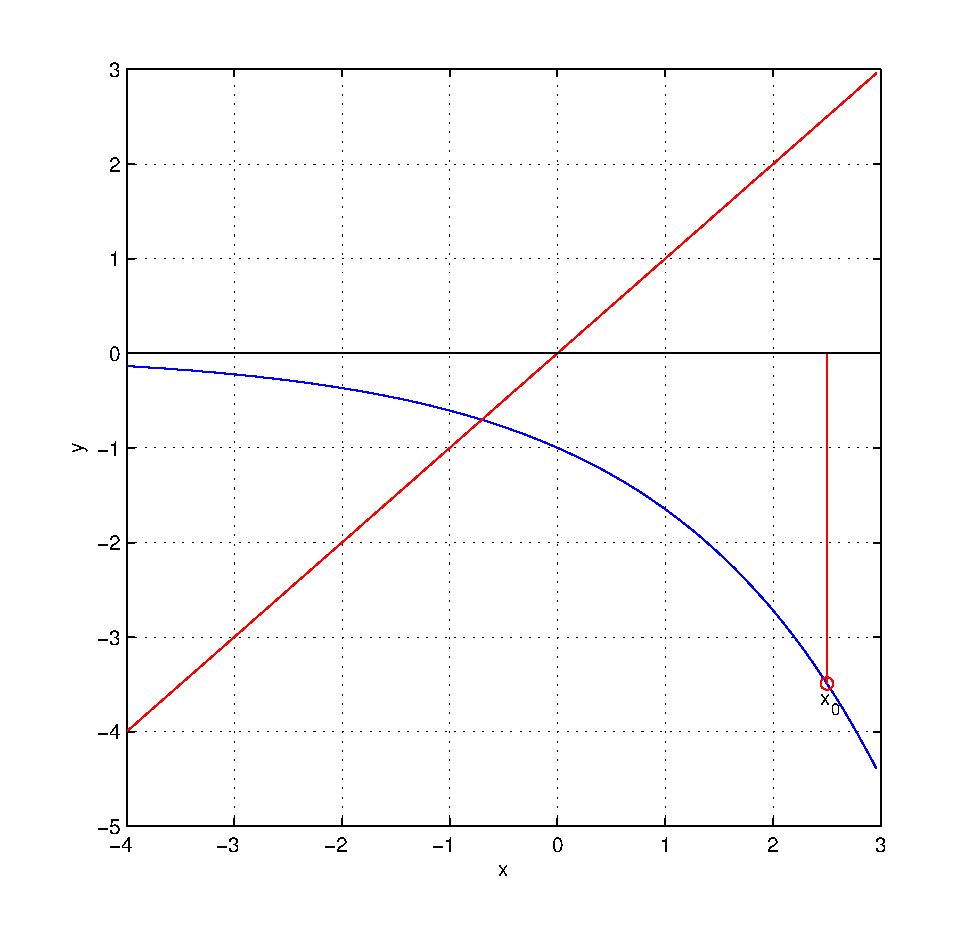
\includegraphics[width=6.6cm]{pfijo3.pdf}} \qquad
\subfigure[iteracion 1]{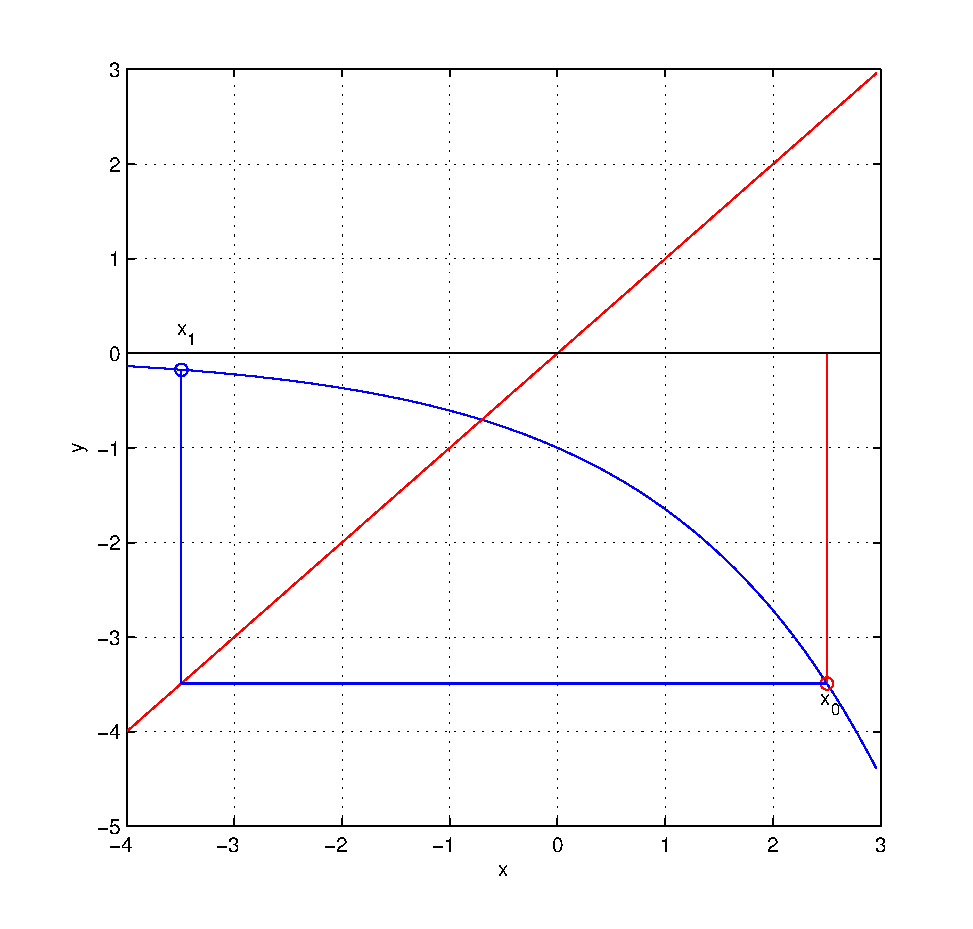
\includegraphics[width=6.5cm]{pfijo4.pdf}}\\
\subfigure[iteración 2]{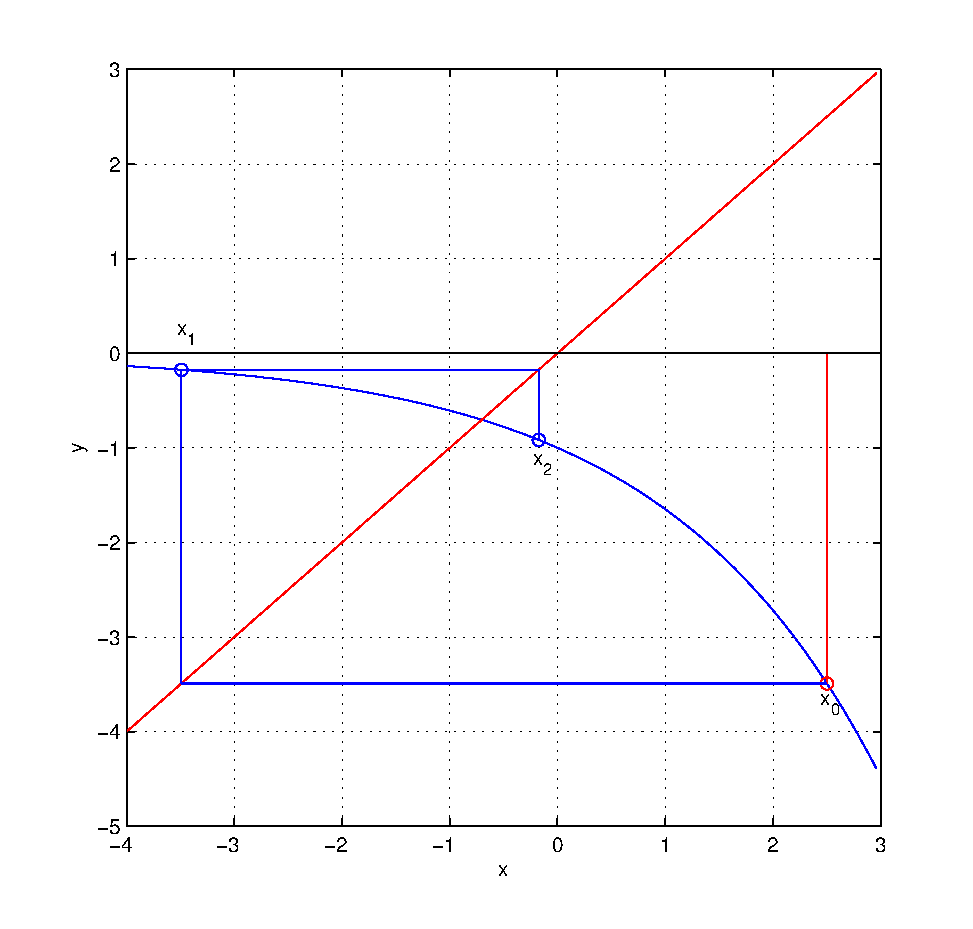
\includegraphics[width=6.5cm]{pfijo5.pdf}}\qquad
\subfigure[iteración 3]{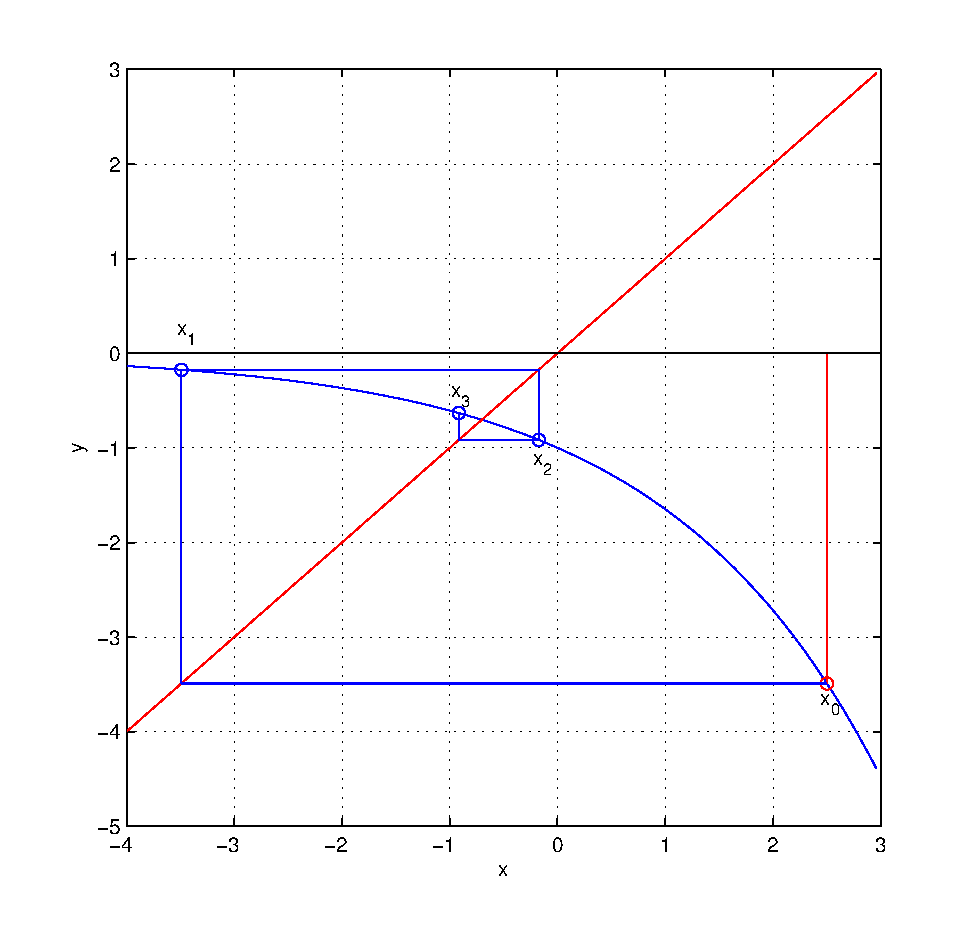
\includegraphics[width=6.5cm]{pfijo6.pdf}}\\
\subfigure[iteración 4]{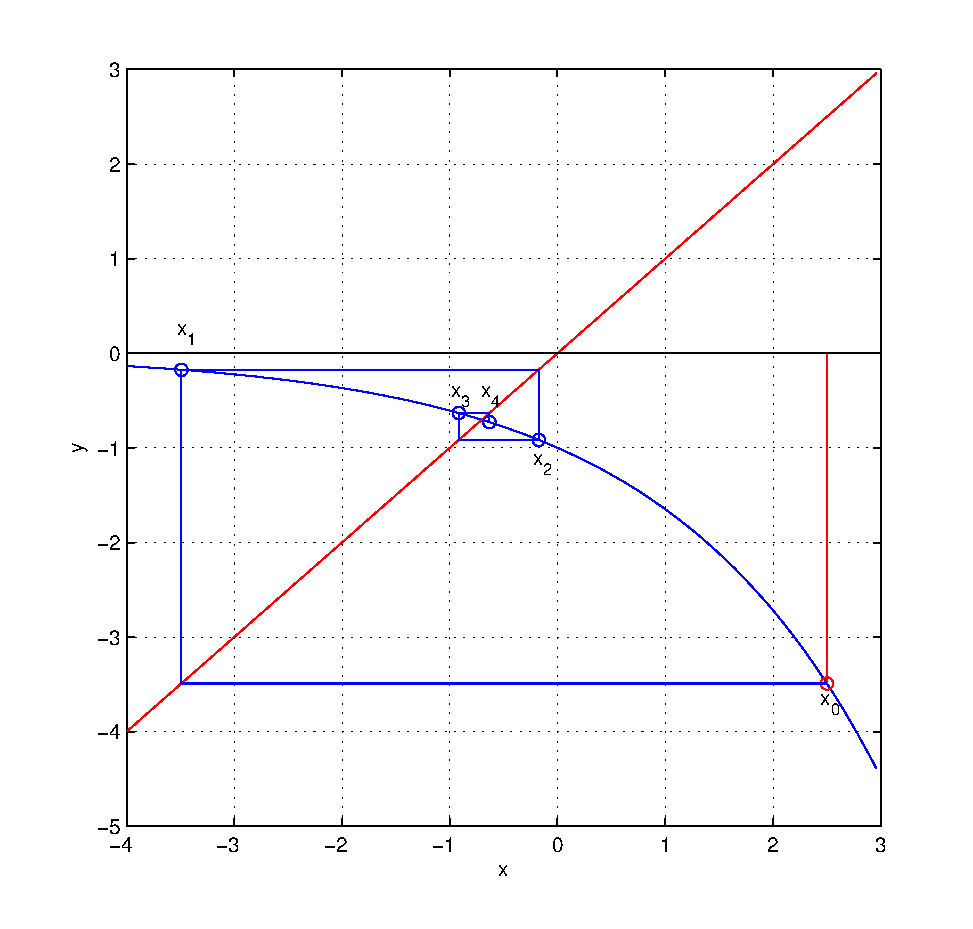
\includegraphics[width=6.5cm]{pfijo7.pdf}}\qquad
\subfigure[iteración 5 \label{fig:pfijo25}]{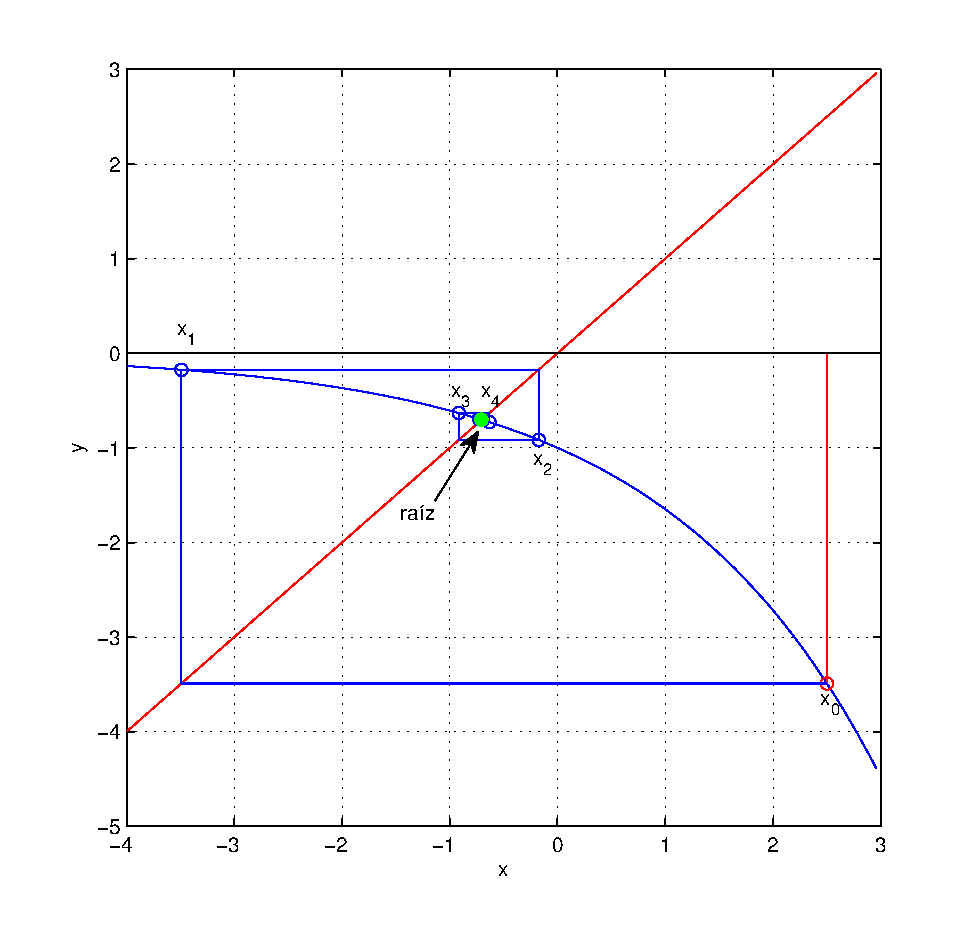
\includegraphics[width=6.5cm]{pfijo8.pdf}}
\caption{proceso de obtención de la raíz de la función $f(x)=e^x-x^2$ aplicando el método del punto fijo sobre la función $g(x)=-\sqrt{e^x}$}.
\label{fig:pfijo2}
\end{figure}

Si tratamos de emplear la función $g(x)=ln(x^2)$ para obtener la raíz, observamos que la función no cumple el teorema para ningún intervalo que contenga la raíz. 

La figura \ref{fig:pfijo03} muestra la función $g(x)$, la recta $y=x$ y la evolución del algoritmo tras cuatro evaluaciones. Es fácil deducir que el algoritmo saltará de la rama positiva a la negativa y de ésta volverá a saltar de nuevo a la positiva. 

\begin{figure}[h]
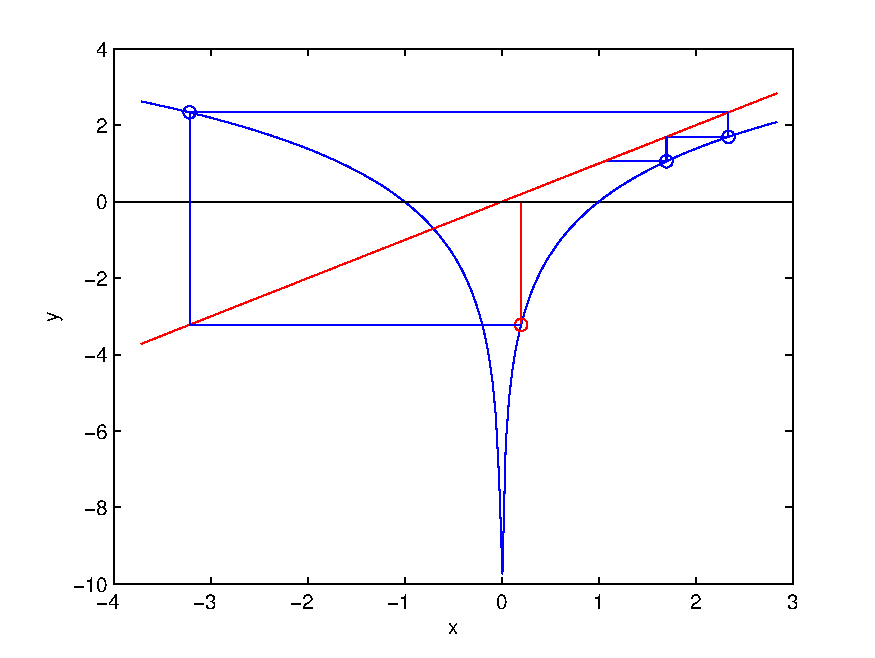
\includegraphics[width=14cm]{p1fijo0.pdf}
\caption{primeras iteraciones de la obtención de la raíz de la función $f(x)=e^x-x^2$ aplicando el método del punto fijo sobre la función $g(x)=ln(x^2)$.}
\label{fig:pfijo03}
\end{figure}

La función presenta una asíntota vertical en el $0$. Si se empieza desde $x_0=0$, $x_0=1$ 0 $x_0=-1$ el algoritmo no converge, puesto que la función diverge hacia $-\infty$. Para el resto de los valores, la función oscila entre una rama y otra. Si en alguna de las oscilaciones acierta a pasar suficientemente cerca del punto fijo, $x_n-x_{n-} \leq tol$, el algoritmo habrá aproximado la raíz, aunque propiamente no se puede decir que converja.

 La figura \ref{fig:pfijo41}, muestra la evolución del algoritmo, tomando como punto inicial $x_0=-0.2$.  Tras 211 iteraciones el algoritmo 'atrapa la raíz'. En este caso la tolerancia se fijó en $tol=0.01$.  
 
 La gráfica \ref{fig:pfijo42} muestra una ampliación de \ref{fig:pfijo41} en la que pueden observarse en detalles los valores obtenidos para las dos últimas iteraciones. Las dos líneas horizontales de puntos marcan los límites $\text{raíz}\pm tol$. 
 
 El algoritmo se detiene porque la diferencia entre los valores obtenidos en las dos últimas iteraciones caen dentro de la tolerancia. El valor obtenido en la penúltima iteración, que proviene de la rama positiva de la función $g(x)$ cae muy cerca del punto fijo. El último valor obtenido, se aleja de hecho del valor de la raíz, respecto al obtenido en la iteración anterior, pero no lo suficiente como para salirse de los límites de la banda marcada por la tolerancia. Como resultado, se cumple la condición de terminación y el algoritmo se detiene.  
 
 Si disminuimos el valor de la tolerancia, no podemos garantizar que el algoritmo converja. De hecho, si trazamos cuales habrían sido los valores siguientes que habría tomado la solución del algoritmo, caso de no haberse detenido, es fácil ver que se alejan cada vez más de la raíz.  De nuevo habrá que esperar a que cambie de rama y vuelva  a pasar otra vez cerca del punto fijo para que haya otra oportunidad de que el algoritmo \emph{atrape} la solución.
 
  La gráfica \ref{fig:pfijo43} muestra la evolución del error en función del número de iteración. Como puede observarse, el error oscila de forma caótica de una iteración a la siguiente. De hecho, el estudio de las sucesiones de la forma $x_{n+1}=g(x_n)$ constituyen uno de los puntos de partidas para la descripción y el análisis de los llamados sistemas caóticos. 

Uno sencillo, pero muy interesante es el de la ecuación logística discreta, $x_{n+1}=R\cdot (1-x_n)\cdot x_n$. Esta ecuación muestra un comportamiento muy distinto, según cual sea el valor de $R$ y el valor inicial $x_0$ con el que empecemos a iterar.
 
 

\begin{figure}[h]
\centering
\subfigure[Evolución del algoritmo durante 211 iteraciones \label{fig:pfijo41}]{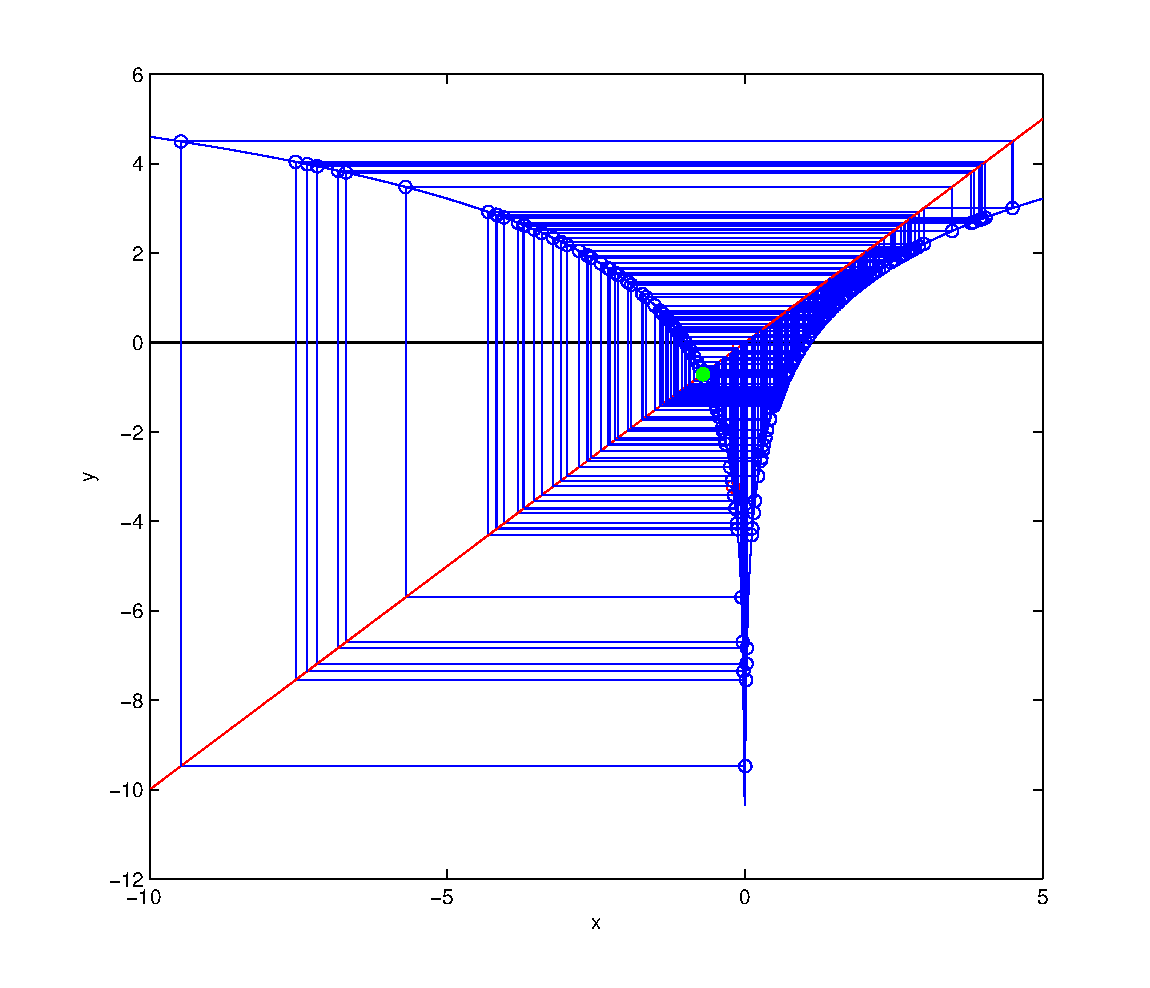
\includegraphics[width=7cm]{p2fijo1.pdf}} \qquad
\subfigure[Vista detallada de las ultimas iteraciones de \ref{fig:pfijo41} \label{fig:pfijo42}]{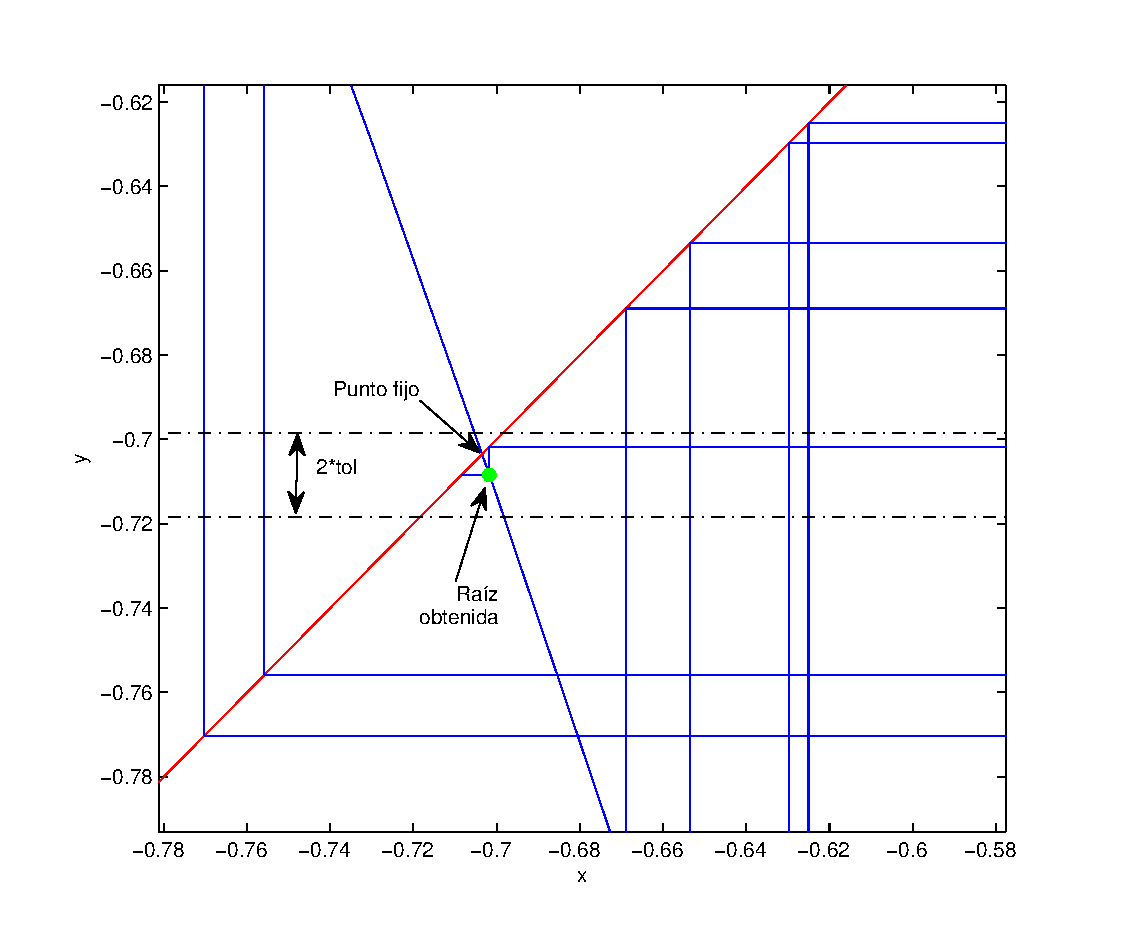
\includegraphics[width=7cm]{p2fijo1d2.eps}}\\
\subfigure[Evolución del error \label{fig:pfijo43}]{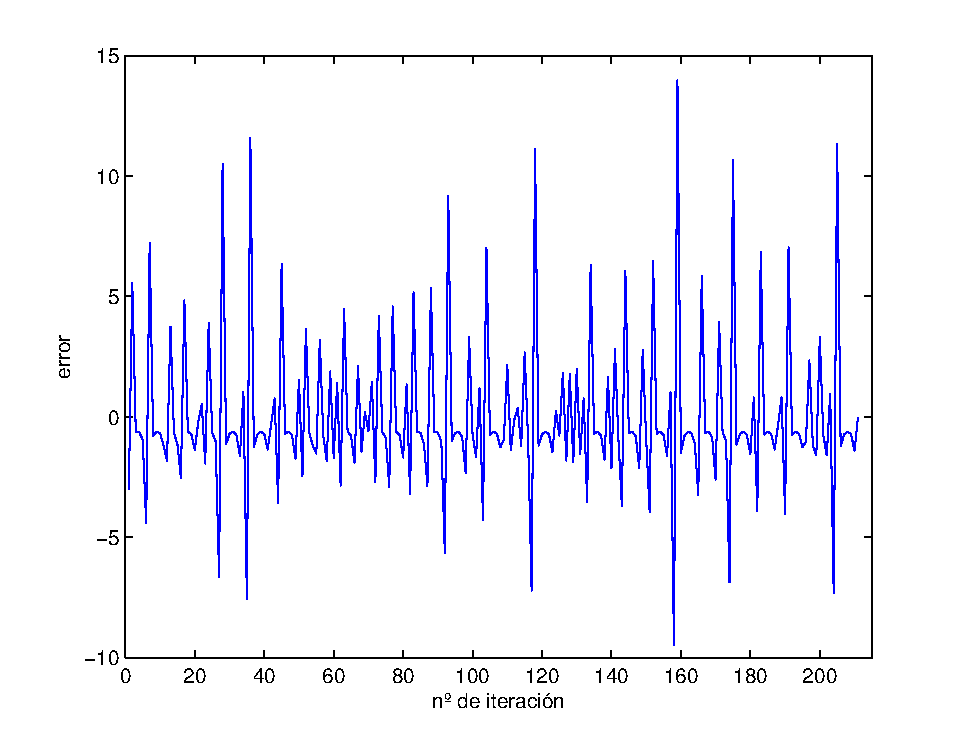
\includegraphics[width=7.2cm]{p2fijo1e.pdf}}

\caption{proceso de obtención de la raíz de la función $f(x)=e^x-x^2$ aplicando el método del punto fijo sobre la función $g(x)=ln(x^2)$, el método oscila sin converger a la solución.}
\label{fig:pfijo4}
\end{figure}

Por último, si empleamos la función $g(x)=\frac{e^x}{x}$, no se cumple el teorema de punto fijo en ningún punt. En este caso, el algoritmo diverge siempre.  La figura \ref{fig:pfijo5} muestra la evolución del algoritmo del punto fijo para esta función. Se ha elegido un punto de inicio $x_0=-0.745$, muy próximo al valor de la raíz, para poder observar la divergencia de las soluciones obtenidas con respecto al punto fijo. Como puede verse, el valor de $x_n$ cada vez se aleja más de la raíz. LA solución oscila entre un valor que cada vez se aproxima más a cero y otro que tiende hacia $-\infty$. Si se deja aumentar suficientemente el número de iteraciones, llegará un momento en que se producirá un error de desbordamiento. 

A diferencia de lo que sucedía en la elección de $g(x)=ln(x^2)$, en este caso, el algoritmo no oscila entre las dos ramas. Si empezamos en la rama de la derecha, eligiendo un valor positivo para $x_0$, el algoritmo diverge llevando las soluciones hacia $+\infty$. Es un resultado esperable, ya que dicha rama no tiene ningún punto fijo.

\begin{figure}
\centering
\subfigure[valor inicial]{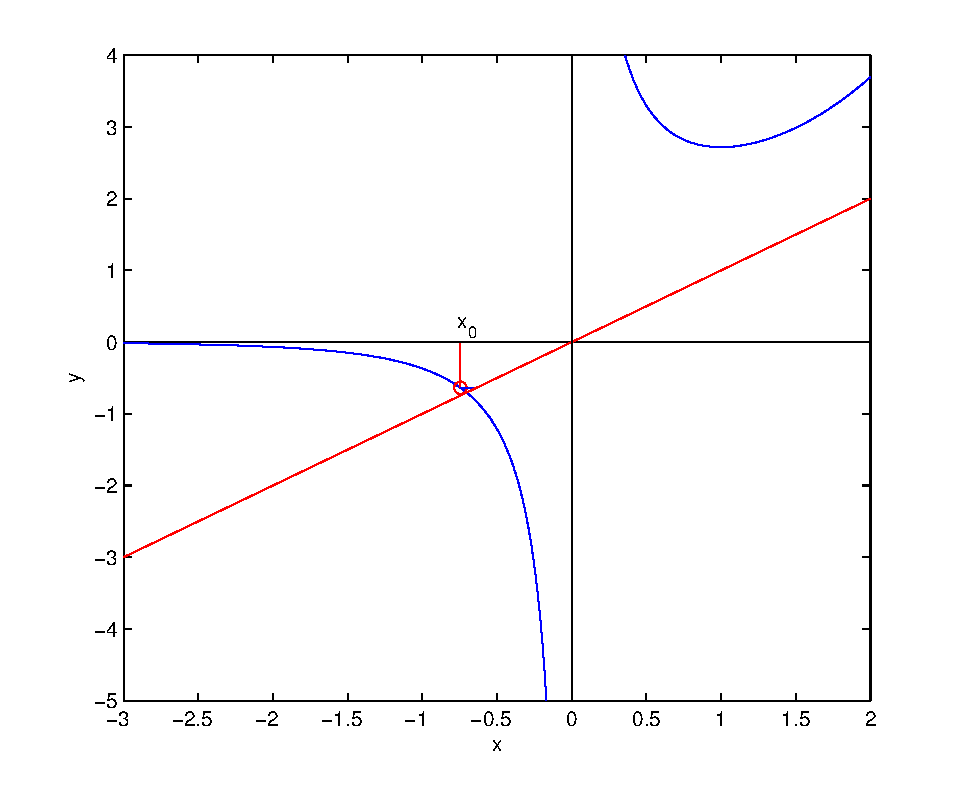
\includegraphics[width=7cm]{p3fijo0.pdf}} \qquad
\subfigure[iteracion 1]{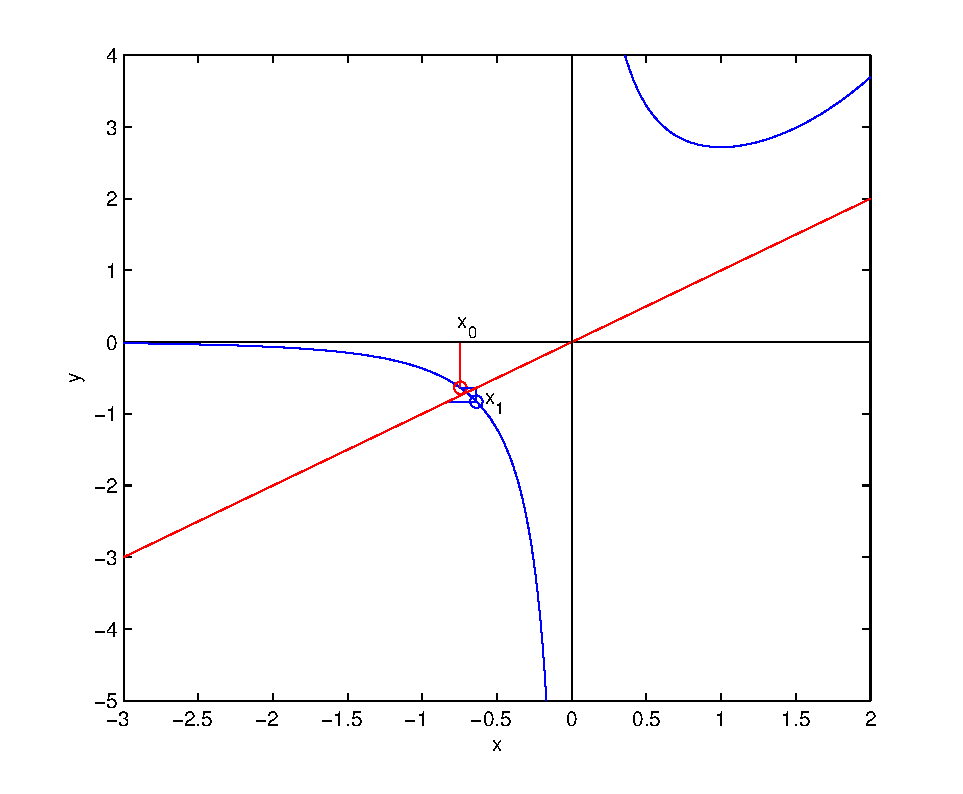
\includegraphics[width=7cm]{p3fijo1.pdf}}\\
\subfigure[iteración 2]{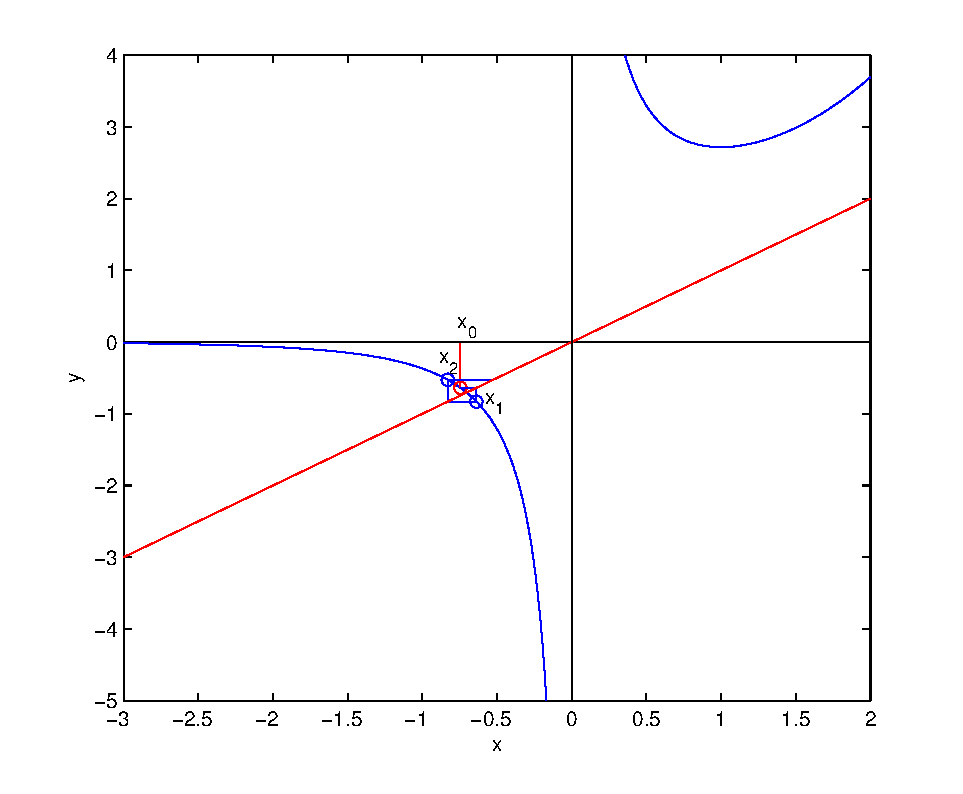
\includegraphics[width=7cm]{p3fijo2.pdf}}\qquad
\subfigure[iteración 3]{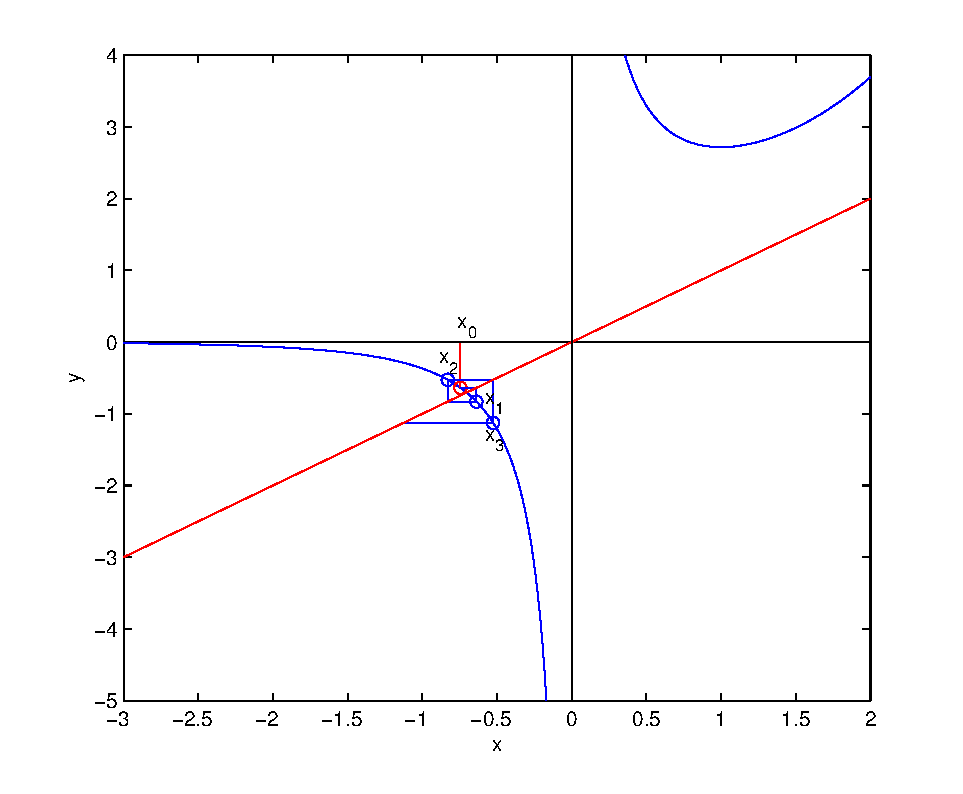
\includegraphics[width=7cm]{p3fijo3.pdf}}\\
\subfigure[iteración 4]{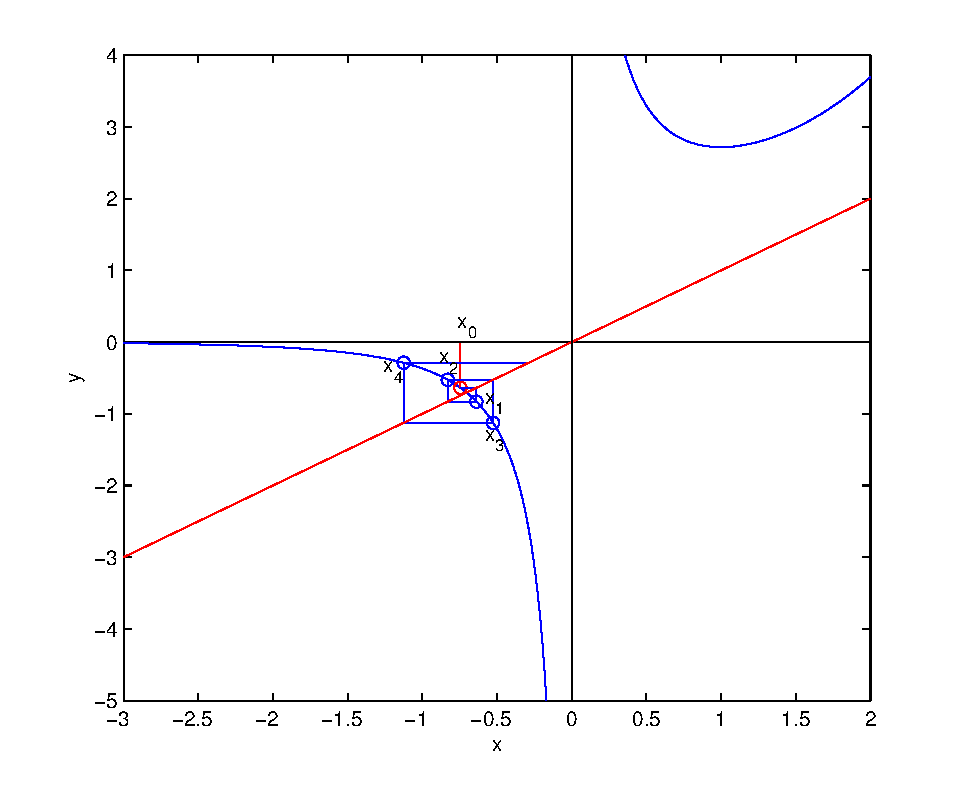
\includegraphics[width=7cm]{p3fijo4.pdf}}\qquad
\subfigure[iteración 5]{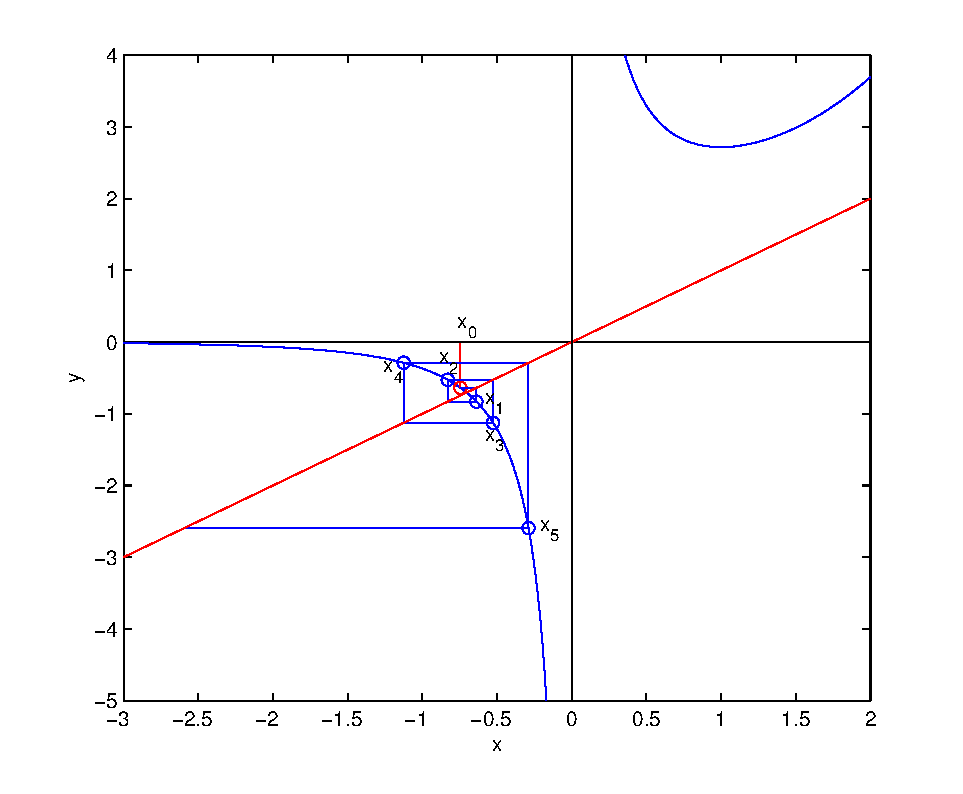
\includegraphics[width=7cm]{p3fijo5.pdf}}

\caption{proceso de obtención de la raíz de la función $f(x)=e^x-x^2$ aplicando el método del punto fijo sobre la función $g(x)=\frac{e^x}{x}$, el método diverge rápidamente.}
\label{fig:pfijo5}
\end{figure}

\section{Cálculo de raíces de funciones con Matlab.}

Matlab suministra funciones propias para calcular raíces de funciones.  Las dividiremos en dos grupos. En primer lugar estudiaremos la función de Matlab \texttt{fzero} y después veremos un conjunto de funciones específicas para manejar polinomios.

\subsection{La función de Matlab \texttt{fzero.}}

La función \texttt{fzero} permite obtener la raíz de una función cualquiera real $f(x):\mathbb{R} \rightarrow \mathbb{R}$. \texttt{fzero}, es una función especial, ya que opera sobre otras funciones, podemos considerarla como una \emph{función de funciones}. Las funciones ordinarias actúan sobre variables, a lo largo de los capítulos anteriores hemos visto como asignar valores y \emph{variables de entrada} a las funciones y también cómo guardar los resultados obtenidos de las funciones en \emph{variables de salida}.

Matlab suministra varios mecanismos, para indicar a \texttt{fzero} ---y en general a cualquier \emph{función de funciones}--- la función sobre la que queremos que actúe. Veremos a continuación algunos de los más comunes.

\paragraph{\emph{handle} de una función.}\index{"@ |emph{handle} de una función} El primer mecanismo, es asociar a una función un nombre de variable especial. Hasta ahora, siempre hemos empleado las variables para guardar en ellas valores numéricos o caracteres. Sin embargo Matlab permite guardar también funciones en una variable. Estas variables, reciben el nombre de \emph{handles}. Veamos un ejemplo. Si escribimos en la ventana de comandos, 

\begin{verbatim}
>> sn =@sin
sn = 
    @sin
\end{verbatim}

Matlab asocia a la nueva variable \texttt{sn} la función seno (\texttt{sin}). Para indicar a Matlab que la nueva variable es el \emph{handle} de una función es imprescindible emplear el símbolo @, después del símbolo de asignación $=$.

Si pedimos a Matlab que nos muestre qué variables tiene en el \emph{workspace},

\begin{verbatim}
>> whos
  Name      Size            Bytes  Class          Attributes

  sn      1x1                32  function_handle              

\end{verbatim}

Matlab nos indica que se ha creado una variable \texttt{sn}, cuya clase es \texttt{function\_handle}. Esta variable tiene propiedades muy interesantes: por una parte, podemos manejarla como si se tratara de la función seno, asignando valores de entrada, y guardando el resultado en una variable de salida, 
\begin{verbatim}
>> x=sn(pi/2)
x =
     1
\end{verbatim}

Pero además podemos usarla como variable de entrada para otra función, tal y como se muestra en el siguiente código,

% \begin{lstlisting}
% function pinta_funcion(fun,intervalo)
% % Esta función dibuja la gráfica de una funcion cualquiera (fun) en un
% % itervalo dado (intervalo). fun debe ser un handle de la función que se
% % quiere pintar. intervalo debe ser un vector que contenga los extremos del
% % intervalo que se desea pintar.

% % Construimos cien puntos en el intevalo dado,
% x=linspace(intervalo(1),intervalo(2),100);

% % calculamos el valor de la funcion en los puntos del intervalo,
% y=fun(x);

% % dibujamos la gráfica
% plot(x,y)
% \end{lstlisting}

La función \texttt{pinta\_funcion} nos dibujará la gráfica de cualquier función en el intervalo indicado. p realizar ara ello bastará crear un \emph{handle} de la función que se quiere dibujar y pasarlo a la función \texttt{pinta\_fun} como una variable de entrada. Así por ejemplo, si escribimos en Matlab,

\begin{verbatim}
>>sn=@sin
>>pinta_funcion(sn,[-pi/2,pi/2])
\end{verbatim}

Se obtendrá la gráfica de la función seno en el intervalo pedido.

Podemos asignar \emph{handles} no solo a las funciones internas de Matlab sino a cualquier función que escribamos. Por ejemplo, en los métodos descritos más arriba para obtener raíces de funciones, usamos la función $f(x)=e^x-x^2$ como función de prueba. podemos crear un fichero que implemente esta función,

\begin{lstlisting}
function y=prueba(x)
% esta es una funcioncilla de prueba para los algoritmos de obtención de
% raíces
y=exp(x)-x.^2;
\end{verbatim}

Si guardamos el fichero, con el nombre prueba.m en el directorio de trabajo, podemos ahora asignar un \emph{handle} a nuestra función,
\begin{verbatim}
mifuncion=@prueba 
\end{verbatim}

Y a continuación, podemos emplear el programa \texttt{pinta\_fun} para representa la función en un intervalo, por ejemplo $[-2 2]$ que contenga la raíz,

\begin{verbatim}
pinta_funcion(mifuncion,[-2 2])
\end{verbatim} 

El resultado se muestra en la figura \ref{fig:handle}

\begin{figure}[h]
\centering
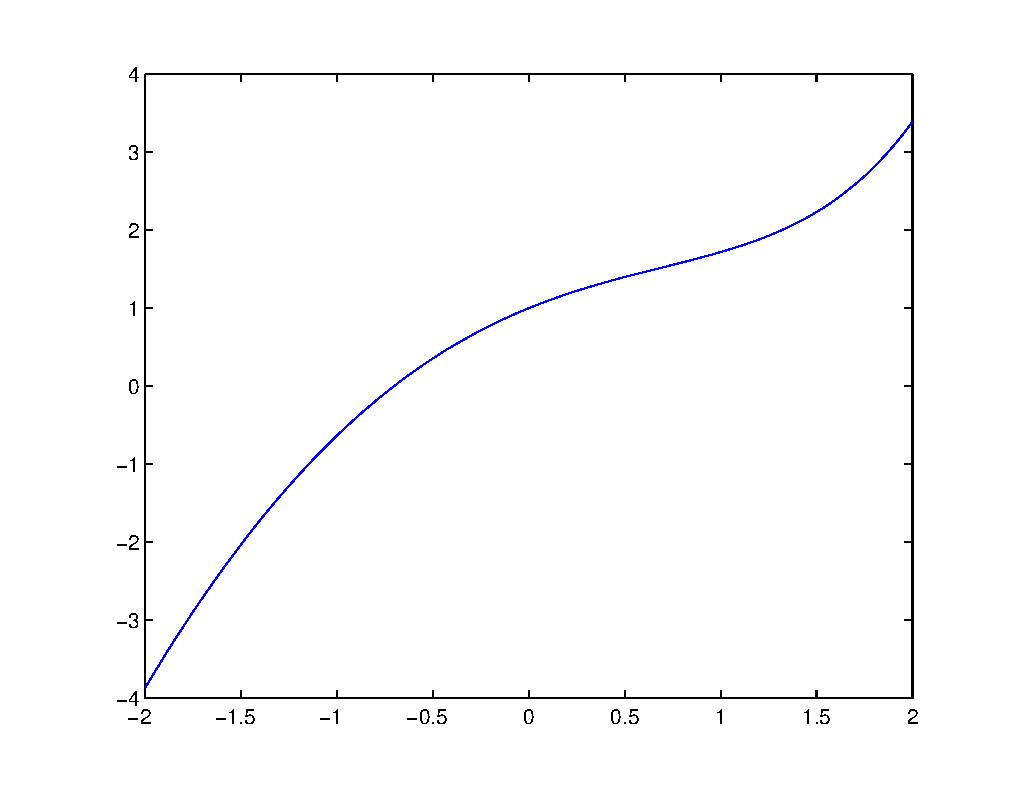
\includegraphics[width=8cm]{handle.eps}
\caption{Gráfica de la función $f(x)=e^x-x^2$, obtenida mediante \texttt{pinta\_funcion}.}
\label{fig:handle}
\end{figure}

\paragraph{la función \texttt{feval} de Matlab.} Esta función suministra un método indirecto para calcular los resultados de una función cualquiera.  Su sintaxis es la siguiente,
\begin{verbatim} 
[y1, y2, ..., ym]=feval('fun', x1, x2, ...,xn)
\end{verbatim}

donde \texttt{fun} representa el nombre de la función que se desea evaluar, \texttt{x1, x2,...,xn}, son la variables de entrada empleadas por la función \texttt{fun}, y \texttt{y1, y2, ...,ym} representan sus variables de salida. Es importante destacar que el nombre de la función que se desea evaluar hay que introducirlo entre comillas simples. Así por ejemplo si escribimos,

 \begin{verbatim}
>> y=feval('sin',x)
y =
     1
>> 
\end{verbatim}
obtenemos el mismo resultado que empleando la función \texttt{sin} directamente para calcular  el valor del seno de $\pi/2$,
\begin{verbatim}
>> x=pi/2;
>> y=sin(x)
y =
     1
>> 
\end{verbatim}
 realizar 



\texttt{feval} suministra un método alternativo al uso de \emph{handles} para crear y manejar \emph{funciones de funciones}. Para ver un ejemplo, el siguiente código muestra una versión alternativa del programa \texttt{pinta\_funcion}, empleando la función \texttt{feval},

\begin{lstlisting}
function pinta_funcion2(fun,intervalo)
% Esta función dibuja la gráfica de una funcion cualquiera (fun) en un
% itervalo dado (intervalo). fun debe ser una cadena de caractéres que contengan exáctamente el nombre de la función (fun) que se 
% quiere pintar. intervalo debe ser un vector que contenga los extremos del
% intervalo que se desea pintar.

% Construimos cien puntos en el intevalo dado,
x=linspace(intervalo(1),intervalo(2),100);

% calculamos el valor de la funcion en los puntos del intervalo, EMPLEANDO LA FUNCION feval
y=feval(fun,x);

% dibujamos la gráfica
plot(x,y)
\end{lstlisting}

Para representar la función seno en el intervalo $-\frac{\pi}{2}, \frac{\pi}{2}$, empleando esta nueva función, introducimos en Matlab,

\begin{verbatim}
>> pinta_funcion2('sin',[-pi/2,pi/2])
\end{verbatim}
 realizar 
También podemos crear una variable alfa-numérica con el nombre de la función seno, y pasar directamente la variable creada,

\begin{verbatim}
>> funcion='sin'
>> pinta_funcion2(funcion,[-pi/2,pi/2])
\end{verbatim}

Al igual que en el caso del uso de \texttt{handles} podemos emplear la función \texttt{feval} con funciones creadas por el usuario, por ejemplo podemos representar nuestra función \texttt{prueba}, introducida anteriormente, 

\begin{verbatim}
>>pinta_funcion2('prueba',[-2 2])
\end{verbatim}

El resultado sería de nuevo la figura \ref{fig:handle}.  Una última propiedad importante de la función \texttt{feval} es que también admite que indiquemos la función a evaluar mediante un \emph{handle}. Sí volvemos al último ejemplo, podríamos haber construido un \emph{handle} para la función \texttt{prueba},
\begin{verbatim}
>>mf=@prueba
>>pinta_funcion2(mf,[-2 2])
\end{verbatim} 

Obtendríamos una vez más el mismo resultado.

\paragraph{Funciones \emph{inline}.} \index{Funciones! \emph{inline}} Las funciones \emph{inlin realizar e} suministran un tercer mecanismo en Matlab para manejar una función de modo que sirva de \emph{variable}  a otra función. Las funciones \emph{inline} tienen una peculiaridad con respecto a las funciones que hemos visto hasta ahora; no se guardan en ficheros .m sino directamente en el \emph{Workspace}. Las funciones \emph{inline} solo existen mientras dura la sesión de Matlab en que se crearon, aunque es posible guardarlas en ficheros .mat y volver a cargarlas en Matlab, como se haría con cualquier otra variable.

Para crear una función \emph{inline} se emplea el comando \texttt{inline}. En su forma más sencilla, el comando debe emplear como variable de entrada una expresión entre comillas simples que represente la expresión matemática de la función. Por ejemplo si queremos hacer una versión \emph{inline} de la función \texttt{prueba},
\begin{verbatim}
>> fun=inline('exp(x)-x.^2')
fun =
     Inline function:
     fun(x) = exp(x)-x^2
\end{verbatim}

Para calcular el valor de la función en un punto, la función \emph{inline} se maneja de  modo análogo a cualquier otra función ordinaria.

\begin{verbatim}
>> y=fun(2)
y =
   3.3891
\end{verbatim}

Como en el caso del uso de \texttt{handles}, la variable creada mediante una función \emph{inline} realizar , hace referencia a una función y puede ser empleada como variable  de entrada por otras funciones. Por ejemplo, podríamos emplear directamente nuestra primera versión del programa para pintar funciones, \texttt{pitan\_funcion} para obtener la gráfica de nuestra función de prueba $f(x)=e^x-x^2$,

\begin{verbatim}
>>funcion=inline('exp(x)-x.^2')
>>pinta_funcion(funcion,[-2 2])
\end{verbatim}

Una vez que hemos visto distintos métodos para manejar una función como variable de entrada de otra función, volvamos a la función \texttt{fzero}. En su forma más sencilla, \texttt{fzero} admite como variable de entrada, una función expresada mediante un \texttt{handle}, mediante su nombre escrito entrecomillas o bien construida como función \emph{inline}. Además es preciso introducir una segunda variable que puede ser un punto $x_0$ próximo a la raíz de la función o bien un vector $[a b]$ que defina un intervalo que contenga una raíz. La función \texttt{fzero}, devuelve como variable de salida el valor aproximado de la raíz. Si \texttt{fzero} no es capaz de encontrar la raíz de la función, devolverá NaN. Veamos un ejemplo con la función contenida en el fichero, prueba.m, descrito más arriba,

\begin{enumerate}
\item Empleando un \emph{handle} y un punto próximo a la raíz,
\begin{verbatim}
>> hndl=@prueba
hndl = 
    @prueba
>> raiz=fzero(hndl,2)
raiz =
  -0.703467422498392
\end{verbatim}
\item Empleando un \emph{handle} y un intervalo que contenga la raíz,
\begin{verbatim}
>> raiz=fzero(hndl,[-2 2])
raiz =
  -0.703467422498392
\end{verbatim}

\item Empleando el nombre de la función entre comillas y un punto cercano a la raíz,
\begin{verbatim}
>> raiz=fzero('prueba',2)
raiz =
  -0.703467422498392
\end{verbatim}

\item  Empleando el nombre de la función entre comillas y un intervalo que contenga la raíz,
\begin{verbatim}
>> raiz=fzero('prueba',[-2 2])
raiz =
  -0.703467422498392
\end{verbatim}

\item Usando una función \emph{inline} y un punto cercano a la raíz,
\begin{verbatim} realizar 
>> finl=inline('exp(x)-x.^2')
finl =
     Inline function:
     finl(x) = exp(x)-x.^2

>> raiz=fzero(finl,2)
raiz =
  -0.703467422498392
\end{verbatim}

\item Usando una función \emph{inline} y un intervalo que contenga la raíz, 
\begin{verbatim}

>> raiz=fzero(finl,[-2 2])
raiz =
  -0.703467422498392
\end{verbatim}
\end{enumerate} 

La función \texttt{fzero}, tiene muchas posibilidades de ajuste de la precisión, del método que emplea internamente para buscar la raíz, etc. Para obtener una visión mas completa de su uso, consultar la ayuda de Matlab.

\subsection{Cálculo de raíces de polinomios.} \index{Polinomios}

Matlab tiene un conjunto de funciones especialmente pensadas para  manejar polinomios. En primer lugar, en Matlab es habitual representar los polinomios mediante vectores cuyos elementos, son los coeficientes del polinomio ordenados de mayor a menor grado. Así por ejemplo, el polinomio. $y=2x^3+3x^2+4x+1$ se representa mediante el vector, $p1=[2\ 3\ 4\ 1]$,  el polinomio $y=3x^4+2x^2+6x$ se representa mediante el vector,  $p2=[3\ 0\ 2\ 6\ 0]$ y, en general, el polinomio $y(x)=a_nx^n+a_{n-1}x^{n-1}+\cdots+a_2x^2+a_1x+a_0$  se representa mediante el vector $p=[a_n\ a_{n-1}\ \cdots\ a_2\ a_1\ a_0]$. Si al polinomio le falta algún o algunos términos, el elemento correspondiente toma el valor $0$ en el vector que representa el polinomio.

Veamos a continuación un conjunto de funciones de Matlab, especialmente pensadas para manejar polinomios,

\paragraph{La función \texttt{roots}.} \index{Polinomios!Raíces de un polinomio}Esta función calcula las raíces de un polinomio de grado $n$ a partir de los coeficientes del polinomio, contenidos en un vector como los que acabamos de describir. La sintaxis es: \texttt{raices=roots([vector de coeficientes])}. veamos un ejemplo. Dado el polinomio $y(x)=x^3-6^2+11x-6$ lo expresaríamos en Matlab como,

\begin{verbatim}
>> p=[1 -6 11 -6]
\end{verbatim}

Y obtendríamos sus raíces como,

\begin{verbatim}
>> raices=roots(p)
raices =
    3.0000
    2.0000
    1.0000

\end{verbatim}

Matlab devuelve todas las raíces del polinomio en un único vector, tanto las reales como las complejas. Como por ejemplo en el caso del polinomio $y(x)=x^2+2x+1$

\begin{verbatim}
>> p=[1 2 3]
p =
     1     2     3
>> raices=roots(p)
raices =
  -1.0000 + 1.4142i
  -1.0000 - 1.4142i
\end{verbatim}

\paragraph{la función \texttt{poly}.} Esta función podría considerarse la opuesta a la anterior; dado un vector que contiene las raíces de un polinomio, nos devuelve los coeficientes del polinomio correspondiente, Por ejemplo si definimos el vector de raíces, 
\begin{verbatim}
>>raices=[3 2 1]
\end{verbatim}
podemos obtener los coeficientes del polinomio que posee esas raíces como,
\begin{verbatim}
>> raices=[1 2 3]
raices =
     1     2     3
>> coef=poly(raices)
coef =
     1    -6    11    -6
\end{verbatim}

Es decir, las raíces pertenecen al polinomio, $y(x)=x^3-6x^2+11x-6$.

\paragraph{la función \texttt{polyval}.}\index{Polinomios!valor de un polinomio en un punto} Esta función calcula el valor de un polinomio en un punto.  Para ello es preciso darle un vector con los coeficientes del polinomio ---definido igual que en los casos anteriores--- y un segundo vector con los puntos para los que se quiere calcular el valor del polinomio,

\begin{verbatim}
>> coef=[1 2 3 4]
coef =
     1     2     3     4
>> x=2
x =
     2
>>y= polyval(coef,x)
y =
    26
>> x=[1:10]º
x =
     1     2     3     4     5     6     7     8     9    10
>> y=polyval(coef,x)
y =
  Columns 1 through 6
          10          26          58         112         194         310
  Columns 7 through 10
         466         668         922        1234
\end{verbatim}  
 

En este ejemplo se ha obtenido con \texttt{polyval} el valor del polinomio $y(x)=x^3+2x^2+2x+4$ primero para el punto $x=2$ y después para los puntos $x=[1\ 2\ 3\ 4\ 5\ 6\ 7\ 8\ 9\ 10]$.

\paragraph{La función \texttt{conv}.} \index{Polinomios!Producto de polinomios}Calcula el producto de dos polinomios. Cada polinomio se representa mediante un vector de coeficientes y la función \texttt{conv} devuelve un vector con los coeficientes del polinomio producto. Por ejemplo, si multiplicamos   el polinomio $y_1=x+2$ por el polinomio $y_2=x-1$  obtendremos como resultado, $p=y_1\cdot y_2=x^2+x-2$,  

\begin{verbatim}
>> y1=[1 2]
y1 =
     1     2
>> y2=[1 -1]
y2 =
     1    -1
>> p=conv(y1,y2)
p =
     1     1    -2
\end{verbatim}

\section{Cálculo de raices con la precisión máxima}
Como ya se vio en la sección \ref{errn} todos los números que empleamos en un ordenador están sometidos a errores a causa del tamaño finito de los registros empleados para guardarlos. Cualquier número que queramos representar ha de aproximarse por un número máquina. Por lo tanto, en vez de buscar la aproximación a la raiz de una función con una tolerancia dada, podemos hallarla con la máxima precisión que nos permita la representación numérica empleada. Esta precisión máxima está relacionada con el \texttt{epsilon} del computador ya que la distancia entre dos números consecutivos es el épsilon multiplicado por dos elevado al exponente del número. De esta manera, por muchas iteraciones que hagamos la mejor aproximación que vamos a poder obtener de una raiz la obtendremos cuando el intervalo en el que se busca la raiz queda reducido a \texttt{eps} y por lo tanto no es posible reducirlo aún más. 

En Matlab el comando  \texttt{eps} nos devuelve justo esa distancia entre dos números de coma flotante consecutivos:

\begin{verbatim}
>> eps(1)

ans =

2.220446049250313e-16

>> eps(1e10)

ans =

1.907348632812500e-06

>> eps(1e-10)

ans =

1.292469707114106e-26

\end{verbatim}

Podemos usar \texttt{eps} para establecer la condición de parada de los algoritmos de búsqueda de raices. Para el caso del método de la bisección se puede modificar el diagrama de flujo según se indica en la figura \ref{fig:dfbisecprecmax}
	
\begin{figure}[h]
	\centering
	\begin{tikzpicture}
	%\usetikzlibrary{shapes.geometric}
	\path (5,0) node(a) [rectangle,draw=blue, very thick,align=center,rounded corners]{Partimos de $[a,b]$\\ con\\ $f(a)\cdot f(b)<0$}
	(5,-2) node(b)[rectangle,draw=blue, thick,rounded corners]{Calculamos $c=\frac{a+b}{2}, f(c)$}
	(5,-4) node(c)[diamond,aspect=3,draw=red,thick]{es $\vert a-b \vert < \text{eps(a)}$?}
	(9,-4) node(d)[rectangle,draw=blue,align=center,very thick, rounded corners]{convergencia:\\ terminar}
	(5,-6) node(e)[diamond,aspect=3,draw=red,thick]{es $f(a)\cdot f(c) < 0$?}
	(9.5,-6) node(f)[rectangle,draw=blue,thick,rounded corners,align=center]{$b=c$\\$f(b)=f(c)$}
	(5,-8) node(g)[rectangle,draw=blue,thick,rounded corners,align=center]{$a=c$\\$f(a)=f(c)$};
	\draw[blue,-latex](a.south)--(b);
	\draw[blue,-latex](b.south)--(c);
	\draw[blue,-latex](c.east)--(d);
	\draw (7.5,-4)node[above]{Sí};
	\draw[blue,-latex](c.south)--(e);
	\draw (5,-5)node[right]{No};
	\draw[blue,-latex](e.east)--(f);
	\draw (8,-6)node[above]{Sí};
	\draw[blue,-latex](e.south)--(g);
	\draw (5,-7.2)node[right]{No};
	\draw[blue,-latex](g.south)|-(2,-9)|-(b);
	\draw[blue,-latex](f.east)-|(11,-2)--(b);
	\end{tikzpicture}
	\caption{Diagrama de flujo del método de la bisección con precisión máxima}
	\label{fig:dfbisecprecmax}
\end{figure}

Es más, en el método de la bisección se puede calcular en función del intervalo inicial el número de iteraciones necesario para alcanzar la máxima precisión, puesto que en cada iteración el intervalo se reduce a la mitad. Si llamamos $d$ al intervalo de partida $d=\vert a-b \vert$, en la iteración $n$ la longitud del intervalo será $\frac{d}{2^{n-1}}$. Se alcanzará el intervalo mínimo posible cuando su longitud sea la de \texttt{eps}. Pero según se explicaba en la sección \ref{errn} el valor de \texttt{eps} es igual a $2$ elevado al número de bits de la mantisa. En el caso de un número de doble precisión la mantisa tiene $52$ bits y por lo tanto:

\begin{equation*}
\frac{\vert d \vert}{2^{n-1}}<2^{-52} 
\end{equation*}

Y despejando y tomando logaritmos:

\begin{equation*}
n > \log_{2}(\vert d \vert)+53
\end{equation*}

Para métodos que no parten de un intervalo sino de un punto inicial, como el de Newton-Raphson o el del punto fijo también puede buscarse la raiz empleando \texttt{eps}, de manera que se alcanzará la precisión máxima cuando el intervalo comprendido entre dos soluciones obtenidas en iteraciones consecutivas sea del tamaño de \texttt{eps}. 

\section{Ejercicios}
\begin{enumerate}
\item Crea una función en matlab que implemente el método de  la bisección para obtener la raíz de una función cualquiera $y = f(x)\vert\  x, y \in \mathbb{R}$. La función deberá admitir como variables de entrada, la función $f(x)$, un intervalo de búsqueda $[a,b]$, un número máximo de iteraciones, $nmax$, a realizar y la tolerancia $tol$ o error máximo admisible para la solución obtenida. Así mismo la función deberá devolver como como variables de salida, el valor aproximado obtenido para la raíz $r$, el error cometido $f(r)$ y el número de iteraciones empleado para alcanzar la solución. 

Aplica el programa creado a la función de ejemplo empleada empleada en el manual, $f(x) = e^x-x^2$, para comprobar que funciona correctamente.

\item Crea una función en matlab que implemente el método de  interpolación lineal para obtener la raíz de una función cualquiera $y = f(x)\vert\  x, y \in \mathbb{R}$. La función deberá admitir como variables de entrada, la función $f(x)$, un intervalo de búsqueda $[a,b]$, un número máximo de iteraciones, $nmax$, a realizar y la tolerancia $tol$ o error máximo admisible para la solución obtenida. Así mismo la función deberá devolver como como variables de salida, el valor aproximado obtenido para la raíz $r$, el error cometido $f(r)$ y el número de iteraciones empleado para alcanzar la solución.

Aplica el programa creado a la función de ejemplo empleada empleada en el manual, $f(x) = e^x-x^2$, para comprobar que funciona correctamente.

\item Crea una función en matlab que implemente el método de  Newton-Raphson para obtener la raíz de una función cualquiera $y = f(x)\vert\  x, y \in \mathbb{R}$. La función deberá admitir como variables de entrada, la función $f(x)$ y su función derivada $f'(x)$, un punto inicial de búsqueda $x_0$, un numero máximo de iteraciones, $nmax$, a realizar y la tolerancia $tol$ o error máximo admisible para la solución obtenida. Así mismo la función deberá devolver como como variables de salida, el valor aproximado obtenido para la raíz $r$, el error cometido $f(r)$ y el número de iteraciones empleado para alcanzar la solución.

Aplica el programa creado a la función de ejemplo empleada empleada en el manual, $f(x) = e^x-x^2$, para comprobar que funciona correctamente.

\item Crea una función en matlab que implemente el método de la secante para obtener la raíz de una función cualquiera $y = f(x)\vert\  x, y \in \mathbb{R}$. La función deberá admitir como variables de entrada, la función $f(x)$ y su función derivada $f'(x)$, dos punto iniciales de búsqueda $x_0,\ x_1$, un numero máximo de iteraciones, $nmax$, a realizar y la tolerancia $tol$ o error máximo admisible para la solución obtenida. Así mismo la función deberá devolver como como variables de salida, el valor aproximado obtenido para la raíz $r$, el error cometido $f(r)$ y el número de iteraciones empleado para alcanzar la solución.

Aplica el programa creado a la función de ejemplo empleada empleada en el manual, $f(x) = e^x-x^2$, para comprobar que funciona correctamente.
\item Crea una función en matlab que implemente el método del punto fijo para obtener la raíz de una función cualquiera $y = f(x)\vert\  x, y \in \mathbb{R}$. La función deberá admitir como variables de entrada, la función auxiliar $g(x)$, necesaria para aplicar el método, un punto inicial de búsqueda $x_0$, un numero máximo de iteraciones, $nmax$, a realizar y la tolerancia $tol$ o error máximo admisible para la solución obtenida. Así mismo la función deberá devolver como como variables de salida, el valor aproximado obtenido para la raíz $r$, el error cometido $f(r)$ y el número de iteraciones empleado para alcanzar la solución.

Aplica el programa creado a la función de ejemplo empleada empleada en el manual, $f(x) = e^x-x^2$, empleando para ello los tres ejemplos de funciones auxiliare $g(x)$ propuestos en la sección \ref{pfijo}. Comprueba que se cumple en cada caso lo expuesto en dicha sección.

\item Se quiere aproximar el valor de $\pi$ utilizando las dos siguientes funciones:
\begin{equation*}
y=\cos(x)+1
\end{equation*}
\begin{equation*}
y=\cos(x/2)
\end{equation*}
\begin{enumerate}
\alph{enumii}
\item \label{it1}Dibuja las dos funciones y sus derivadas en el intervalo $[\frac{\pi}{2},\frac{3\pi}{2}]$.
\item Aplica el método de la secante para cada función, tomando como punto de partida  $x_0=3$ y obteniendo en ambos caso la solución con una tolerancia de 0.01. Elige para $x_1$ un valor que consideres adecuado.\\
El programa utilizado deberá añadir al gráfico obtenido en  \ref{it1}), un punto en la posición $(x_i,y_i)$ que represente el valor obtenido de la raíz en cada iteración $i$.
\item Compara el número de iteraciones que se necesitan en cada caso para obtener la solución.
\end{enumerate}
\item El método de Steffensen, permite disminuir el número de iteraciones empleadas para obtener una raíz empleando el método del punto fijo.

El algoritmo calcula cada iteración usando dos pasos intermedios de acuerdo con el siguiente procedimiento,

% \begin{lstlisting}
% while{condición} 
%   x0 = x
%   x1 = g(x0)
%   x2 = g(x1)
%   x  = x0 - (x1 -x0)^2/(x2 - 2x1 + x0)
% end
% \end{lstlisting}

Donde $g(x)$ representa la función auxiliar de la que se busca el punto fijo.


Dada la función,

\begin{equation*}
y= x^2-2x-3
\end{equation*} 

se le puede aplicar el método del punto fijo a  partir de dos reordenaciones distintas:
\begin{equation}
x^2-2x-3=0 \Rightarrow x=\sqrt{2x+3}
\end{equation}
y
\begin{equation}
x^2-2x-3=0 \Rightarrow x=\frac{3}{x-2}
\end{equation}
\begin{enumerate}
\item Aplica el método del punto fijo, tomando como punto de partida $x_0=4$, mediante ambas reordenaciones. Calcula en ambos casos la raíz con una tolerancia de $0.0001$. Indica en cada caso: el valor de la raíz y el número de interaciones empleadas.  ¿Son razonables los resultados?

\item Repite el calculo empleando ahora el método de Steffensen y comprueba si emplea o no menos iteraciones que el punto fijo.
\end{enumerate}

\item Un objeto se mueve de acuerdo con la siguiente ley:
\begin{equation}
x_1 = 3t^6 - 2t^5 + t + 25
\end{equation}
Donde  $t$ representa el tiempo en segundos y $x_1$ la posición del objeto en metros y \\
 Un segundo objeto sale en persecución del primero en el instante de tiempo $t=0$. Su ley del movimiento es:
\begin{equation}
x_2 = 4t^6
\end{equation}
\begin{enumerate}
\item Dibuja en un mismo gráfica la posición en función del tiempo para los dos móviles, de modo que se observe el punto de alcance. (1 punto) 
\item Calcula, empleando el método de la bisección o el de \emph{regula falsi},  el instante de tiempo y la posición en que el segundo móvil alcanza al primero (2 puntos)
\end{enumerate}

\item La distribución de Maxwell, 
\begin{equation}
f(v) = \sqrt{\frac{2}{\pi}}\left( \frac{m}{kT}\right)^{3/2}v^2e^{-\dfrac{\scriptstyle mv^2}{\scriptstyle 2kT}},
\end{equation}
da la probabilidad de que una partícula de un gas se mueva con velocidad $v$. Donde $m$ es la masa de la partícula en Kg, $T$ la temperatura en grados Kelving del gas y k $=1.380649\times 10^{-23} \text{JK}^{-1}$ la constante de Boltzmann. 
\begin{enumerate}
\item  \label{eje91}Dibuja una gráfica de la distribución de Maxwell a temperatura ambiente T $= 300$K para el Nitrógeno N$_2$  cuya masa molecular vale $m = 4.65 \times 10^{-26}	\text{Kg}$.
\item \label{eje92}Calcula a dicha temperatura cual es el valor más probable de la velocidad de una partícula.
\item Calcula cuánto hay que bajar la temperatura para que la probabilidad de encontrar una partícula con la velocidad calculada en el apartado \ref{eje92} valga 0.001. Dibuja sobre la misma gráfica del ejercicio \ref{eje91} la distribución de Maxwell del Nitrógeno para esta nueva temperatura. 

\end{enumerate}

\end{enumerate}

\section{Test del curso 2020/2021}
\begin{enumerate}
\item Una señal de FM, viene representada por la función
\begin{equation}
	x(t) = 2\cos\left(\pi \, t+ \frac{3}{2}\sin\left(\frac{\pi}{2} \, t\right)\right).
\end{equation}
\begin{enumerate}
	\item \textbf{1 punto. }Dibuja la función en el intervalo $[0,\pi]$ Emplea para ello valores equiespaciados $0.01\pi$.
	\item \textbf{3 puntos. }Calcula los tres primeros instantes de tiempo en los que la señal vale cero, empleando para ello el método de la bisección. Elige en cada caso los intervalos adecuados. Obtén los resultados empleando una tolerancia $tol=0.001$ e indica el número de iteraciones empleadas.
\end{enumerate}

\item  Han Solo ha situado en reposo al Halcón Milenario en un punto del universo alejado de toda galaxia. Tras dejar a Chewbacca en una nave auxiliar, Han pone en marcha los motores (modelo \emph{Girodyne SRB42 Sublight Engine Thrusters}) y el Halcón acelera con una aceleración uniforme $a_0 = 3\times10^3\ m/s^2$. Chewabaca --que no estudió físicas--  desconoce la Teoría de la Relatividad, y por lo tanto piensa que puede calcular la posición $x_{cl}$ con respecto del Halcón empleando la función clásica del movimiento rectilíneo uniformemente acelerado
\begin{equation}
	x_{cl}(t) =\frac{1}{2}a_0t^2.
\end{equation}
		En realidad el Halcón no puede acelerar indefinidamente (sobrepasaría la velocidad de la luz, cosa imposible con los \emph{Sublight Engine Thrusters}), por lo que la posición real $x_{rel}$ a la que se encuentra viene expresada por
\begin{equation}
	x_{rel}(t) = \frac{c^2}{a_0}\sqrt{1 + \frac{a_0^2\,t^2}{c^2}} -\frac{c^2}{a_0}, 
\end{equation}
		donde $c \approx 3\times 10^8 m/s$ representa la velocidad de la luz en el vacío. 

		En los siguientes pasos vamos a calcular cuanto tiempo transcurre hasta que Chewbacca comete un error de un miliparsec\footnote{$1\,\text{Parsec} \approx 3\times 10^{16}m$.} en el cálculo de la posición del Halcón.

\begin{enumerate}
	\item {\bf 2 puntos.} Define la función de error $e(t) = x_{cl}(t) - x_{rel}(t)$ y simplifícala con los datos numéricos dados. Acto seguido, reescribe la función error como $e(t) = t - g(t)$ para poder aplicar más adelante el algoritmo del punto fijo. Con una sola descomposición de $e(t)$ es suficiente. De hecho, quédate únicamente con aquella que tenga una $g(t)$ más simple según tu criterio.

	\item {\bf 1.5 puntos.} Dibuja en una misma gráfica la función $y = g(t)$ y la bisectriz del primer cuadrante $y = t$, y comprueba que $g(t)$ tiene efectivamente un punto fijo. Para la gráfica escoge el intervalo de tiempo $[0, \quad 3 \times 10^5]$ segundos con intervalos de $1\times 10^4$ segundos.
	\item {\bf 2.5 puntos.} Emplea el método del punto fijo para obtener el tiempo en el que el error en posición alcanza un valor igual a un miliParsec. Da el resultado en días terrestres. Toma como valor inicial $t_0 = 1$ y da el resultado con una tolerancia $tol = 0.1$. Indica el número de iteraciones que ha empleado el método para obtener el resultado.
	\item {\bf Bonus track: 1 punto.} Un Parsec equivale a la distancia desde el Sol a una estrella que, vista desde la Tierra, subtiende un ángulo de paralaje de 1 segundo de grado. Da dos razones por las que el Halcón Milenario nunca pudo atravesar el corredor Kessel en menos de 12 Parsecs, como afirma Han Solo.

\end{enumerate}
\end{enumerate}
